% Options for packages loaded elsewhere
\PassOptionsToPackage{unicode}{hyperref}
\PassOptionsToPackage{hyphens}{url}
%
\documentclass[
]{article}
\usepackage{amsmath,amssymb}
\usepackage{iftex}
\ifPDFTeX
  \usepackage[T1]{fontenc}
  \usepackage[utf8]{inputenc}
  \usepackage{textcomp} % provide euro and other symbols
\else % if luatex or xetex
  \usepackage{unicode-math} % this also loads fontspec
  \defaultfontfeatures{Scale=MatchLowercase}
  \defaultfontfeatures[\rmfamily]{Ligatures=TeX,Scale=1}
\fi
\usepackage{lmodern}
\ifPDFTeX\else
  % xetex/luatex font selection
\fi
% Use upquote if available, for straight quotes in verbatim environments
\IfFileExists{upquote.sty}{\usepackage{upquote}}{}
\IfFileExists{microtype.sty}{% use microtype if available
  \usepackage[]{microtype}
  \UseMicrotypeSet[protrusion]{basicmath} % disable protrusion for tt fonts
}{}
\makeatletter
\@ifundefined{KOMAClassName}{% if non-KOMA class
  \IfFileExists{parskip.sty}{%
    \usepackage{parskip}
  }{% else
    \setlength{\parindent}{0pt}
    \setlength{\parskip}{6pt plus 2pt minus 1pt}}
}{% if KOMA class
  \KOMAoptions{parskip=half}}
\makeatother
\usepackage{xcolor}
\usepackage[margin=1in]{geometry}
\usepackage{color}
\usepackage{fancyvrb}
\newcommand{\VerbBar}{|}
\newcommand{\VERB}{\Verb[commandchars=\\\{\}]}
\DefineVerbatimEnvironment{Highlighting}{Verbatim}{commandchars=\\\{\}}
% Add ',fontsize=\small' for more characters per line
\usepackage{framed}
\definecolor{shadecolor}{RGB}{248,248,248}
\newenvironment{Shaded}{\begin{snugshade}}{\end{snugshade}}
\newcommand{\AlertTok}[1]{\textcolor[rgb]{0.94,0.16,0.16}{#1}}
\newcommand{\AnnotationTok}[1]{\textcolor[rgb]{0.56,0.35,0.01}{\textbf{\textit{#1}}}}
\newcommand{\AttributeTok}[1]{\textcolor[rgb]{0.13,0.29,0.53}{#1}}
\newcommand{\BaseNTok}[1]{\textcolor[rgb]{0.00,0.00,0.81}{#1}}
\newcommand{\BuiltInTok}[1]{#1}
\newcommand{\CharTok}[1]{\textcolor[rgb]{0.31,0.60,0.02}{#1}}
\newcommand{\CommentTok}[1]{\textcolor[rgb]{0.56,0.35,0.01}{\textit{#1}}}
\newcommand{\CommentVarTok}[1]{\textcolor[rgb]{0.56,0.35,0.01}{\textbf{\textit{#1}}}}
\newcommand{\ConstantTok}[1]{\textcolor[rgb]{0.56,0.35,0.01}{#1}}
\newcommand{\ControlFlowTok}[1]{\textcolor[rgb]{0.13,0.29,0.53}{\textbf{#1}}}
\newcommand{\DataTypeTok}[1]{\textcolor[rgb]{0.13,0.29,0.53}{#1}}
\newcommand{\DecValTok}[1]{\textcolor[rgb]{0.00,0.00,0.81}{#1}}
\newcommand{\DocumentationTok}[1]{\textcolor[rgb]{0.56,0.35,0.01}{\textbf{\textit{#1}}}}
\newcommand{\ErrorTok}[1]{\textcolor[rgb]{0.64,0.00,0.00}{\textbf{#1}}}
\newcommand{\ExtensionTok}[1]{#1}
\newcommand{\FloatTok}[1]{\textcolor[rgb]{0.00,0.00,0.81}{#1}}
\newcommand{\FunctionTok}[1]{\textcolor[rgb]{0.13,0.29,0.53}{\textbf{#1}}}
\newcommand{\ImportTok}[1]{#1}
\newcommand{\InformationTok}[1]{\textcolor[rgb]{0.56,0.35,0.01}{\textbf{\textit{#1}}}}
\newcommand{\KeywordTok}[1]{\textcolor[rgb]{0.13,0.29,0.53}{\textbf{#1}}}
\newcommand{\NormalTok}[1]{#1}
\newcommand{\OperatorTok}[1]{\textcolor[rgb]{0.81,0.36,0.00}{\textbf{#1}}}
\newcommand{\OtherTok}[1]{\textcolor[rgb]{0.56,0.35,0.01}{#1}}
\newcommand{\PreprocessorTok}[1]{\textcolor[rgb]{0.56,0.35,0.01}{\textit{#1}}}
\newcommand{\RegionMarkerTok}[1]{#1}
\newcommand{\SpecialCharTok}[1]{\textcolor[rgb]{0.81,0.36,0.00}{\textbf{#1}}}
\newcommand{\SpecialStringTok}[1]{\textcolor[rgb]{0.31,0.60,0.02}{#1}}
\newcommand{\StringTok}[1]{\textcolor[rgb]{0.31,0.60,0.02}{#1}}
\newcommand{\VariableTok}[1]{\textcolor[rgb]{0.00,0.00,0.00}{#1}}
\newcommand{\VerbatimStringTok}[1]{\textcolor[rgb]{0.31,0.60,0.02}{#1}}
\newcommand{\WarningTok}[1]{\textcolor[rgb]{0.56,0.35,0.01}{\textbf{\textit{#1}}}}
\usepackage{longtable,booktabs,array}
\usepackage{calc} % for calculating minipage widths
% Correct order of tables after \paragraph or \subparagraph
\usepackage{etoolbox}
\makeatletter
\patchcmd\longtable{\par}{\if@noskipsec\mbox{}\fi\par}{}{}
\makeatother
% Allow footnotes in longtable head/foot
\IfFileExists{footnotehyper.sty}{\usepackage{footnotehyper}}{\usepackage{footnote}}
\makesavenoteenv{longtable}
\usepackage{graphicx}
\makeatletter
\def\maxwidth{\ifdim\Gin@nat@width>\linewidth\linewidth\else\Gin@nat@width\fi}
\def\maxheight{\ifdim\Gin@nat@height>\textheight\textheight\else\Gin@nat@height\fi}
\makeatother
% Scale images if necessary, so that they will not overflow the page
% margins by default, and it is still possible to overwrite the defaults
% using explicit options in \includegraphics[width, height, ...]{}
\setkeys{Gin}{width=\maxwidth,height=\maxheight,keepaspectratio}
% Set default figure placement to htbp
\makeatletter
\def\fps@figure{htbp}
\makeatother
\setlength{\emergencystretch}{3em} % prevent overfull lines
\providecommand{\tightlist}{%
  \setlength{\itemsep}{0pt}\setlength{\parskip}{0pt}}
\setcounter{secnumdepth}{5}
% definitions for citeproc citations
\NewDocumentCommand\citeproctext{}{}
\NewDocumentCommand\citeproc{mm}{%
  \begingroup\def\citeproctext{#2}\cite{#1}\endgroup}
\makeatletter
 % allow citations to break across lines
 \let\@cite@ofmt\@firstofone
 % avoid brackets around text for \cite:
 \def\@biblabel#1{}
 \def\@cite#1#2{{#1\if@tempswa , #2\fi}}
\makeatother
\newlength{\cslhangindent}
\setlength{\cslhangindent}{1.5em}
\newlength{\csllabelwidth}
\setlength{\csllabelwidth}{3em}
\newenvironment{CSLReferences}[2] % #1 hanging-indent, #2 entry-spacing
 {\begin{list}{}{%
  \setlength{\itemindent}{0pt}
  \setlength{\leftmargin}{0pt}
  \setlength{\parsep}{0pt}
  % turn on hanging indent if param 1 is 1
  \ifodd #1
   \setlength{\leftmargin}{\cslhangindent}
   \setlength{\itemindent}{-1\cslhangindent}
  \fi
  % set entry spacing
  \setlength{\itemsep}{#2\baselineskip}}}
 {\end{list}}
\usepackage{calc}
\newcommand{\CSLBlock}[1]{\hfill\break\parbox[t]{\linewidth}{\strut\ignorespaces#1\strut}}
\newcommand{\CSLLeftMargin}[1]{\parbox[t]{\csllabelwidth}{\strut#1\strut}}
\newcommand{\CSLRightInline}[1]{\parbox[t]{\linewidth - \csllabelwidth}{\strut#1\strut}}
\newcommand{\CSLIndent}[1]{\hspace{\cslhangindent}#1}
\ifLuaTeX
  \usepackage{selnolig}  % disable illegal ligatures
\fi
\usepackage{bookmark}
\IfFileExists{xurl.sty}{\usepackage{xurl}}{} % add URL line breaks if available
\urlstyle{same}
\hypersetup{
  pdftitle={Lineare Regression},
  pdfauthor={Walter Gruber},
  hidelinks,
  pdfcreator={LaTeX via pandoc}}

\title{Lineare Regression}
\author{Walter Gruber}
\date{2025-05-07}

\begin{document}
\maketitle

{
\setcounter{tocdepth}{2}
\tableofcontents
}
\section*{}\label{section}
\addcontentsline{toc}{section}{}


\includegraphics[width=1\textwidth,height=\textheight]{Images/Assumptions.JPG}

\section*{Vorwort}\label{vorwort}
\addcontentsline{toc}{section}{Vorwort}

Dieses Skriptum basiert (großteils) auf Literatur von Andy Field und Rand Wilcox (\citeproc{ref-FieldWilcox.2017}{\&. W. Field A. P. 2017}), David Erceg-Hurn et.al. (\citeproc{ref-Hurn.2008}{Hurn 2008}), Mair (\citeproc{ref-Mair.2020}{Mair 2020}) and Wilcox (\citeproc{ref-Wilcox.2012}{Wilcox 2012}). Teile der hier verwendeten Inhalte wurden unverändert aus der angegebenen Literatur übernommen.

\section*{Einführung}\label{einfuxfchrung}
\addcontentsline{toc}{section}{Einführung}

Kapitel 1: Einführung in die Einfache Lineare Regression

In einer Welt, die zunehmend von Daten geprägt ist, sind statistische Methoden unverzichtbare Werkzeuge, um Muster aufzudecken und fundierte Entscheidungen zu treffen. Die einfache lineare Regression ist eine der grundlegendsten, aber zugleich wirkungsvollsten Techniken in der Statistik. Sie ermöglicht es, den Zusammenhang zwischen zwei quantitativen Variablen zu modellieren und vorherzusagen, wie sich Änderungen in einer unabhängigen Variable auf eine abhängige Variable auswirken.

In diesem Kapitel werden wir die Grundlagen der einfachen linearen Regression erkunden:

\begin{itemize}
\tightlist
\item
  Was bedeutet es, einen linearen Zusammenhang zwischen zwei Variablen zu postulieren?
\item
  Wie wird ein lineares Regressionsmodell aufgestellt und interpretiert?
\end{itemize}

Durch anschauliche Beispiele und Schritt-für-Schritt-Anleitungen (in R) werden wir die Schlüsselkonzepte und mathematischen Grundlagen dieser Methode erläutern.

Ziel ist es, Ihnen ein solides Verständnis für die einfache lineare Regression zu vermitteln, das als Basis für komplexere statistische Analysen dient.

\begin{figure}
\centering

\includegraphics[width=0.3\textwidth,height=\textheight]{Images/RobustHansaPlast.JPG}
\caption{\textbf{Figure 1}: use StatParaPlast to solve all your nasty statistical problems. Look inside the package to disover the fantastic world on NNS (No Nonsense Statistic). Available in different sizes and colors.}
\end{figure}

\part*{PART I: GLM-Assumptions}\label{part-part-i-glm-assumptions}
\addcontentsline{toc}{part}{PART I: GLM-Assumptions}

\section*{Critical Assumptions}\label{critical-assumptions}
\addcontentsline{toc}{section}{Critical Assumptions}

In many fields of psychological research, variants of the general linear model (\emph{GLM}) are used. In this model, an outcome variable \(Y\) is predicted from a \emph{linear} and \emph{additive combination} of one or more predictor variables (\emph{predictors}), i.e.~\(X_1, \cdots, X_n\).

For each predictor, a \emph{parameter} (\(\hat{b}_i\), \emph{slope}) is estimated from the data. This parameter represents the relationship between the predictor and outcome variable if the effects of other predictors in the model are held constant\footnote{ trivial but worthwhile to note at this point: the parameters are estimated based on the observed data. As a consequence we must conclude, that if the data does not represent the outcome in the population, the parameters will NOT represent the relationship between the predictors and the \emph{real world}.}.

There is also a parameter (\(\hat{b}_0\), \emph{constant/intercept}) to estimate the value of the outcome when all predictors are zero.

The errors in prediction are represented by the residuals (\(\varepsilon_i\)), which are (for each observation, \(i\)) the distance between the value of the outcome predicted by the model and the value observed in the data.

\[\begin{array}{c}
  \hat{Y}_i = \hat{b}_0 + \hat{b}_1 \cdot X_{1i} + \cdots + \hat{b}_n \cdot X_{1n} + \varepsilon_i
\end{array}\]

There are two common ways to estimated the parameters \(\hat{b}_k\) with \(k \epsilon \{0,n\}\):

\begin{itemize}
\tightlist
\item
  using \textbf{O}rdinary \textbf{L}east \textbf{S}quares (\href{https://phet.colorado.edu/sims/html/least-squares-regression/latest/least-squares-regression_en.html}{OLS}) estimation: which seeks to minimize the squared errors between the predicted
\item
  \textbf{M}aximum \textbf{L}ikelihood (\textbf{ML}) estimation: which seeks to find the parameter values that maximize the likelihood of the observations.
\end{itemize}

\begin{quote}
The OLS estimator will also be the maximum likelihood estimator (ML), when the assumptions of independent-, homoscedastic- and normally-distributed-errors are met! When these assumptions are not met, the ML estimator will yield different results to the OLS.
\end{quote}

The \textbf{G}eneral \textbf{L}inear \textbf{M}odel (\textbf{GLM}) is a flexible framework through which to predict a continuous outcome variable from predictor variables that are/can be:

\begin{itemize}
\tightlist
\item
  continuous (\emph{regression} or \emph{multiple regression})
\item
  categorical (\emph{ANOVA}) or
\item
  both (\emph{ANCOVA}), or \emph{Moderation-Analysis}, when interactions are modelled.
\end{itemize}

Similarly, experimental designs containing repeated measures and longitudinal data are special cases of a \textbf{multilevel linear model} in which observations (level 1) are nested within participants (level 2). If we include terms that estimate the variance across contexts (e.g., time) in both the constant (\(\zeta_{0j}\)) and model parameters (e.g., \(\zeta_{1j}\)) for each predictor, we get a multilevel model in which observations (\(i\)) are nested within contexts (\(j\)). These contexts could be individuals (e.g., repeated measures designs) or environments (e.g., classrooms).

\[\begin{array}{c}
  \hat{Y}_{ij} = \hat{b}_0 + \hat{b}_1 \cdot X_{ij} + (\zeta_{0i} + \zeta_{1j} \cdot X_{ij} + \varepsilon_{ij})
\end{array}\]

What we must not forget is that they are \emph{all variants of the linear model} and, therefore, \emph{have a common set of underlying assumptions!}. The two main assumptions are:

\begin{enumerate}
\def\labelenumi{\arabic{enumi}.}
\tightlist
\item
  additivity and linearity
\item
  spherical residuals (= independent\footnote{ Independent residuals are ones that are not correlated across observations. Correlation across residuals is known as \emph{autocorrelation}.} and homoscedastic\footnote{ \emph{Homoscedastic} residuals are ones that have the same variance for all observations. Residuals without this property are called \emph{heteroscedastic}.})
\end{enumerate}

\begin{quote}
When applying this models we assume that the outcome variable is linearly related to any predictors and that the best description of the effect of several predictors is that their individual effects can be added together. As such, the \textbf{assumption of additivity and linearity is the most important} because it equates to the general linear model being the best description of the process of interest. When these conditions are met (and residuals have a mean of zero) then the linear model derived from OLS estimation will be a best linear unbiased\footnote{ \textbf{Unbiased} means that the estimator's expected value for a parameter matches the true value of that parameter.} estimator. \textbf{If this assumption is not true then you are fitting the wrong model}.
\end{quote}

To summarize:

\begin{enumerate}
\def\labelenumi{\arabic{enumi}.}
\tightlist
\item
  When data is heteroscedastic, the formula for the variance of the parameters \(\hat{b}_k\) is incorrect.
\item
  Consequently, the estimation of the Standard Error \(SE\) is incorrect.
\item
  Autocorrelation introduces further bias to \(SE\).
\item
  Biased\footnote{ a test statistic is \textbf{biased} if the probability of rejecting the null is not minimized when the null is true.} standard errors have important consequences for significance tests and confidence intervals (CI's) of model parameters (i.e.~CI's can be extremely inaccurate when \(SE\) is biased).
\end{enumerate}

\section*{Normality}\label{normality}
\addcontentsline{toc}{section}{Normality}

Before looking into different problems with normality we shall have a closer look at distributions which seem to be normal but aren't!

\subsection*{Contaminated Normal distributions}\label{contaminated-normal-distributions}
\addcontentsline{toc}{subsection}{Contaminated Normal distributions}

Before we dig into some details let us illustrate the effects of slight depatures form normality. Suppose we sample (an arbitrary variable) from the population of all adults. Within this sample about 10\% are of age 70 and over. Let us assume, that the people younger than 70 have a mean \(\bar{x}_Y = 0\) and a standard deviation of \(sd_Y = 1\). The older people also show a mean of \(\bar{x}_O = 0\), but there standard deviation is much higher, e.g.~\(sd_O = 10\). The following graph shows the standard normal distribution (\emph{black}) vs.~the mixed distribution of our example ({\emph{blue}}). Again, only 10\% of the data for this distribution has a different variance ({\emph{red}}). Do you think these distributions can be considered identical, or at least both of them are normally distributed?

\begin{figure}
\centering
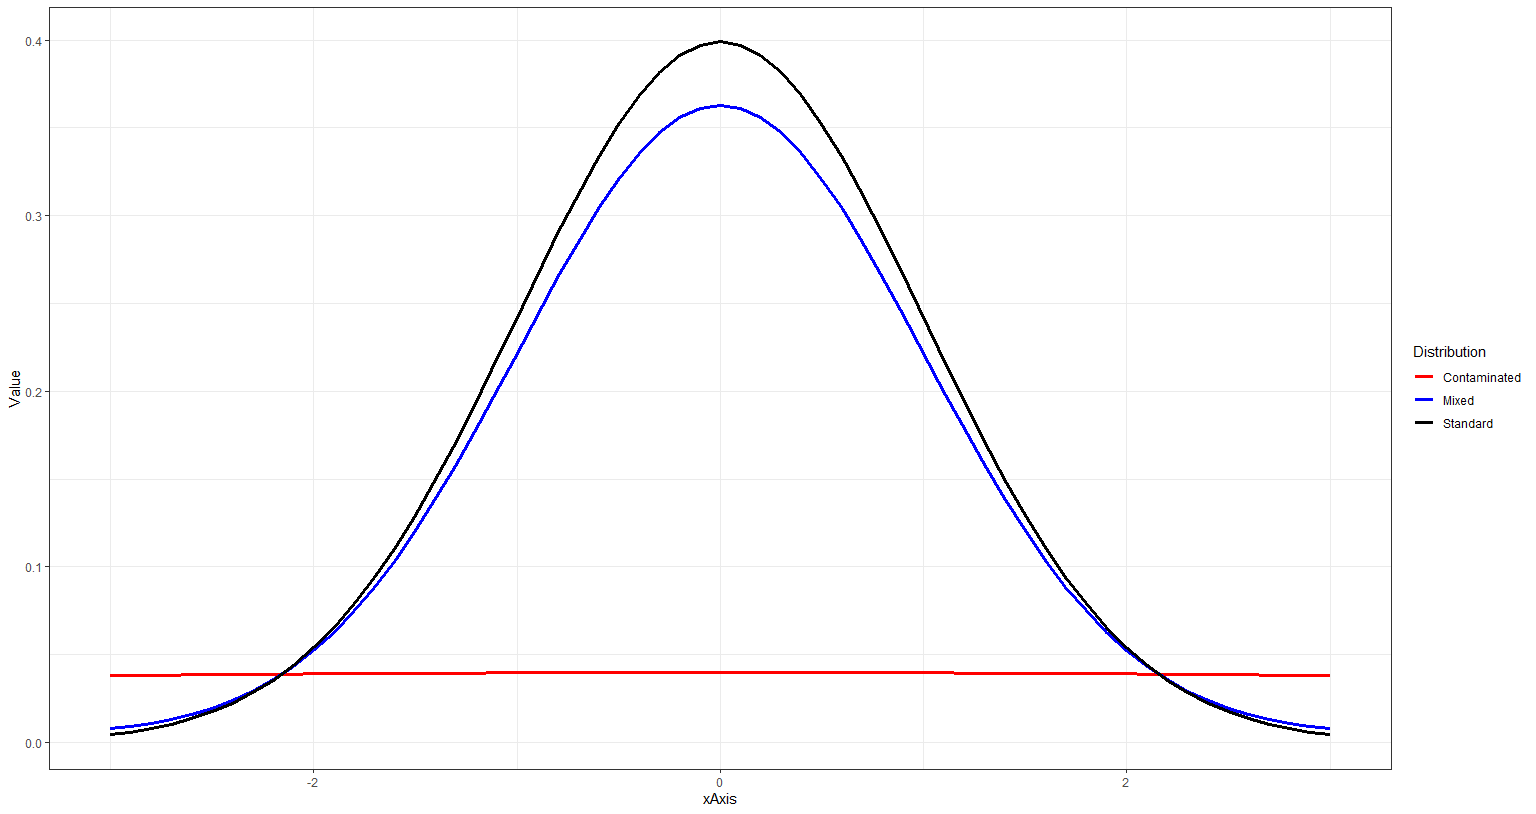
\includegraphics[width=0.5\textwidth,height=\textheight]{Images/Wilcox-2-Contaminated-Full-Plot.jpg}
\caption{Comparison of different normal distributions}
\end{figure}

If we observe such results on representative samples, we could assume, that the entire population has a \emph{mixed}, or \emph{contaminated distribution} with \(\varepsilon = 0.1\) and \(\lambda = 10\). So, in a formal way we would define two independent distributions (\(X, Y\)) with different standard deviations and different sample sizes which are mixed in a distribution \(H\) with the variance of \(Var(H)\), such that:

\[\begin{array}{ccc}
  X            & \approx & N(\mu = 0, sd = 1) \\
  Y            & \approx & N(\mu = 0, sd = \lambda) = N(\mu = 0, sd = 10) \\
  H            & = & (1-\varepsilon) \cdot X + \varepsilon \cdot (x)  = 0.9 \cdot X + 0.1 \cdot Y\\
  \overline{H} & = & E(H) = 0 \\
  Var(H)       & = & E(H^2) \\
  E(H^2)       & = & E(0.9 \cdot X^2 + 0.1 \cdot Y^2 + 2 \cdot X \cdot Y \cdot 0.9 \cdot 0.1) \\
               & = &  0.9 \cdot \underbrace{E(X^2)}_{=1^2} + 0.1 \cdot \underbrace{E(Y^2)}_{=10^2} + 2 \cdot 0.9 \cdot 0.1 \cdot \underbrace{E(X \cdot Y)}_{\text{= Cov(X,Y)=0}} \\
               & = &  0.9 \cdot 1 + 0.1 \cdot 100 = 10.9
\end{array}\]

If we look at the distribution plots, we notice that both (standard normal and contaminated normal) both look very similar. We could conclude, that the contaminated normal is approximating the standard normal distribution to such extent, that we can assume it is also a normal distribution.

\begin{Shaded}
\begin{Highlighting}[]
\NormalTok{  xfrom  }\OtherTok{\textless{}{-}} \SpecialCharTok{{-}}\DecValTok{3}
\NormalTok{  xto    }\OtherTok{\textless{}{-}} \SpecialCharTok{+}\DecValTok{3}
\NormalTok{  Mu     }\OtherTok{\textless{}{-}} \DecValTok{0}
\NormalTok{  SD     }\OtherTok{\textless{}{-}} \DecValTok{1}
\NormalTok{  Epsilon  }\OtherTok{\textless{}{-}} \FloatTok{0.1} \CommentTok{\# percentage of smaller sample with higher std}
\NormalTok{  Lambda }\OtherTok{\textless{}{-}} \DecValTok{10}  \CommentTok{\# standard deviataion of smaller sample}
  \CommentTok{\# x      \textless{}{-} seq(from = xfrom * Lambda, to = xto * Lambda, by = 0.1)}
\NormalTok{  x      }\OtherTok{\textless{}{-}} \FunctionTok{seq}\NormalTok{(}\AttributeTok{from =}\NormalTok{ xfrom, }\AttributeTok{to =}\NormalTok{ xto, }\AttributeTok{by =} \FloatTok{0.1}\NormalTok{)}
\NormalTok{  N      }\OtherTok{\textless{}{-}} \FunctionTok{length}\NormalTok{(x)}
\NormalTok{  Y1     }\OtherTok{\textless{}{-}} \ConstantTok{NULL}
\NormalTok{  Y2     }\OtherTok{\textless{}{-}} \ConstantTok{NULL}
  \CommentTok{\# Y3     \textless{}{-} NULL}
\NormalTok{  CN     }\OtherTok{\textless{}{-}} \ConstantTok{NULL}
  
  \ControlFlowTok{for}\NormalTok{ (i }\ControlFlowTok{in} \DecValTok{1}\SpecialCharTok{:}\NormalTok{N) \{}
\NormalTok{    Y1[i]    }\OtherTok{\textless{}{-}} \FunctionTok{dnorm}\NormalTok{(x[i], }\AttributeTok{mean =}\NormalTok{ Mu, }\AttributeTok{sd =}\NormalTok{ SD) }\CommentTok{\# std. normal component}
\NormalTok{    Y2[i]    }\OtherTok{\textless{}{-}} \FunctionTok{dnorm}\NormalTok{(x[i], }\AttributeTok{mean =}\NormalTok{ Mu, }\AttributeTok{sd =}\NormalTok{ SD}\SpecialCharTok{*}\NormalTok{Lambda) }\CommentTok{\# contamination}
    \CommentTok{\# Y2[i]    \textless{}{-} dnorm(x[i]/Lambda, mean = Mu, sd = SD) \# contamination (same as above)}
\NormalTok{    CN[i] }\OtherTok{\textless{}{-}}\NormalTok{ ((}\DecValTok{1} \SpecialCharTok{{-}}\NormalTok{ Epsilon) }\SpecialCharTok{*}\NormalTok{ Y1[i]) }\SpecialCharTok{+}\NormalTok{ (Epsilon }\SpecialCharTok{*}\NormalTok{ Y2[i])}
\NormalTok{  \}}
\NormalTok{  DF\_CN  }\OtherTok{\textless{}{-}} \FunctionTok{data.frame}\NormalTok{(}\AttributeTok{xAxis =}\NormalTok{ x, }\AttributeTok{Standard =}\NormalTok{ Y1, }\AttributeTok{Contaminated =}\NormalTok{ Y2, }\AttributeTok{Mixed =}\NormalTok{ CN)}
    \CommentTok{\# probability density function (pdf) for one input z{-}value to}
    \CommentTok{\# show the equivalence to the dnorm() function for the same parameters mean}
    \CommentTok{\# and sd.}
    \CommentTok{\# stddev \textless{}{-} 1}
    \CommentTok{\# zwert  \textless{}{-} {-}3}
    \CommentTok{\# Phi \textless{}{-} (1/sqrt(2*pi*stddev\^{}2)) * exp({-}0.5*(zwert/stddev)\^{}2)}
    \CommentTok{\# Y1[1] == Phi}
  \CommentTok{\# ggplot(DF\_CN, aes(x = xAxis)) + }
  \CommentTok{\#   geom\_line(aes(y = Standard), color = "red") + }
  \CommentTok{\#   geom\_line(aes(y = Contaminated), color = "blue") + }
  \CommentTok{\#   geom\_line(aes(y = Mixed), color="black", linetype="twodash") }
  \CommentTok{\#}
  \CommentTok{\# library(tidyverse)}
\NormalTok{  DF\_CN\_P1 }\OtherTok{\textless{}{-}}\NormalTok{ DF\_CN }\SpecialCharTok{\%\textgreater{}\%} 
              \FunctionTok{gather}\NormalTok{(}\AttributeTok{key =} \StringTok{"Distribution"}\NormalTok{, }\AttributeTok{value =} \StringTok{"Value"}\NormalTok{, }\SpecialCharTok{{-}}\NormalTok{xAxis)}
  \CommentTok{\# head(DF\_CN\_P1)}
\NormalTok{  P1 }\OtherTok{\textless{}{-}} \FunctionTok{ggplot}\NormalTok{(DF\_CN\_P1, }\FunctionTok{aes}\NormalTok{(}\AttributeTok{x =}\NormalTok{ xAxis, }\AttributeTok{y =}\NormalTok{ Value)) }\SpecialCharTok{+}
        \CommentTok{\# geom\_line(aes(color = Distribution, linetype = Distribution), size = 1.3) + }
        \FunctionTok{geom\_line}\NormalTok{(}\FunctionTok{aes}\NormalTok{(}\AttributeTok{color =}\NormalTok{ Distribution), }\AttributeTok{size =} \FloatTok{1.3}\NormalTok{) }\SpecialCharTok{+} 
        \FunctionTok{scale\_color\_manual}\NormalTok{(}\AttributeTok{values =} \FunctionTok{c}\NormalTok{(}\StringTok{"red"}\NormalTok{, }\StringTok{"blue"}\NormalTok{, }\StringTok{"black"}\NormalTok{)) }\SpecialCharTok{+}
        \FunctionTok{theme\_bw}\NormalTok{()}
\NormalTok{  DF\_CN\_P1 }\OtherTok{\textless{}{-}} \FunctionTok{subset}\NormalTok{(DF\_CN\_P1, Distribution }\SpecialCharTok{==} \StringTok{"Standard"} \SpecialCharTok{|}\NormalTok{ Distribution }\SpecialCharTok{==} \StringTok{"Mixed"}\NormalTok{)}
\NormalTok{  P2 }\OtherTok{\textless{}{-}} \FunctionTok{ggplot}\NormalTok{(DF\_CN\_P1, }\FunctionTok{aes}\NormalTok{(}\AttributeTok{x =}\NormalTok{ xAxis, }\AttributeTok{y =}\NormalTok{ Value)) }\SpecialCharTok{+}
    \FunctionTok{geom\_line}\NormalTok{(}\FunctionTok{aes}\NormalTok{(}\AttributeTok{color =}\NormalTok{ Distribution), }\AttributeTok{size =} \FloatTok{1.3}\NormalTok{) }\SpecialCharTok{+}
    \FunctionTok{scale\_color\_manual}\NormalTok{(}\AttributeTok{values =} \FunctionTok{c}\NormalTok{(}\StringTok{"blue"}\NormalTok{, }\StringTok{"black"}\NormalTok{)) }\SpecialCharTok{+}
    \FunctionTok{theme\_bw}\NormalTok{()}
\end{Highlighting}
\end{Shaded}

Even so they look like almost identical, they are NOT! Notice the very slight difference at the left and right side (the tails) of the distribution. It might seem just a slight difference, but has in fact a quite dramatic impact on the variance. The variance for the standard normal (black) is 1, whereas for the combined normal (red) the variance is at 10.9 (c.f. to our results above)! We can simulate this effect quite easy - just copy and paste the following code and compare the results:

\begin{Shaded}
\begin{Highlighting}[]
\NormalTok{  NSim }\OtherTok{\textless{}{-}} \DecValTok{50000}
  \FunctionTok{set.seed}\NormalTok{(}\DecValTok{143}\NormalTok{)}
\NormalTok{  Y3 }\OtherTok{\textless{}{-}} \FunctionTok{rnorm}\NormalTok{(NSim, }\AttributeTok{mean =}\NormalTok{ Mu, }\AttributeTok{sd =}\NormalTok{ SD)}
  \FunctionTok{set.seed}\NormalTok{(}\DecValTok{3143}\NormalTok{)}
\NormalTok{  Y4 }\OtherTok{\textless{}{-}} \FunctionTok{rnorm}\NormalTok{(NSim, }\AttributeTok{mean =}\NormalTok{ Mu, }\AttributeTok{sd =}\NormalTok{ SD }\SpecialCharTok{*}\NormalTok{ Lambda)}
\NormalTok{  z  }\OtherTok{\textless{}{-}} \FunctionTok{sample}\NormalTok{(}\FunctionTok{c}\NormalTok{(}\DecValTok{0}\NormalTok{,}\DecValTok{1}\NormalTok{),}
               \AttributeTok{size    =}\NormalTok{ NSim,}
               \AttributeTok{prob    =} \FunctionTok{c}\NormalTok{(}\DecValTok{1}\SpecialCharTok{{-}}\NormalTok{Epsilon, Epsilon),}
               \AttributeTok{replace =} \ConstantTok{TRUE}\NormalTok{)}
\NormalTok{  Hx            }\OtherTok{\textless{}{-}}\NormalTok{ Y3 }\SpecialCharTok{*}\NormalTok{ (}\DecValTok{1}\SpecialCharTok{{-}}\NormalTok{z) }\SpecialCharTok{+}\NormalTok{ Y4 }\SpecialCharTok{*}\NormalTok{ z}
\NormalTok{  DF\_Sim        }\OtherTok{\textless{}{-}} \FunctionTok{data.frame}\NormalTok{(}\AttributeTok{Standard =}\NormalTok{ Y3, }\AttributeTok{Contaminated =}\NormalTok{ Y4, }\AttributeTok{Mixed =}\NormalTok{ Hx)}
\NormalTok{  DF\_Sim\_L      }\OtherTok{\textless{}{-}}\NormalTok{ DF\_Sim }\SpecialCharTok{\%\textgreater{}\%} \FunctionTok{gather}\NormalTok{(}\AttributeTok{key =} \StringTok{"Distribution"}\NormalTok{, }\AttributeTok{value =} \StringTok{"Value"}\NormalTok{)}
\NormalTok{  Res           }\OtherTok{\textless{}{-}} \FunctionTok{summary\_by}\NormalTok{(DF\_Sim\_L,Value }\SpecialCharTok{\textasciitilde{}}\NormalTok{ Distribution, }\AttributeTok{FUN =} \FunctionTok{c}\NormalTok{(mean, var))}
  \FunctionTok{colnames}\NormalTok{(Res) }\OtherTok{\textless{}{-}} \FunctionTok{c}\NormalTok{(}\StringTok{"Distribution"}\NormalTok{, }\StringTok{"Means"}\NormalTok{, }\StringTok{"Variances"}\NormalTok{)}
\NormalTok{  Res[,}\DecValTok{2}\SpecialCharTok{:}\DecValTok{3}\NormalTok{]     }\OtherTok{\textless{}{-}} \FunctionTok{round}\NormalTok{(Res[,}\DecValTok{2}\SpecialCharTok{:}\DecValTok{3}\NormalTok{], }\DecValTok{2}\NormalTok{)}
\NormalTok{  knitr}\SpecialCharTok{::}\FunctionTok{kable}\NormalTok{(Res, }\AttributeTok{caption =} \StringTok{"Results of the simulation. Note the huge difference in the standard and mixed distribution."}\NormalTok{)}
\end{Highlighting}
\end{Shaded}

\begin{table}

\caption{\label{tab:Wilcox-2-Simiulation}Results of the simulation. Note the huge difference in the standard and mixed distribution.}
\centering
\begin{tabular}[t]{l|r|r}
\hline
Distribution & Means & Variances\\
\hline
Contaminated & 0.03 & 100.81\\
\hline
Mixed & -0.03 & 10.87\\
\hline
Standard & -0.01 & 1.00\\
\hline
\end{tabular}
\end{table}

\begin{quote}
In essence, a small proportion of the population of participants can have an inordinately large effect on its value.
\end{quote}

A look at the Q-Q-plot reveals the problem of the mixed distribution in a quite impressive way:

\begin{figure}
\centering
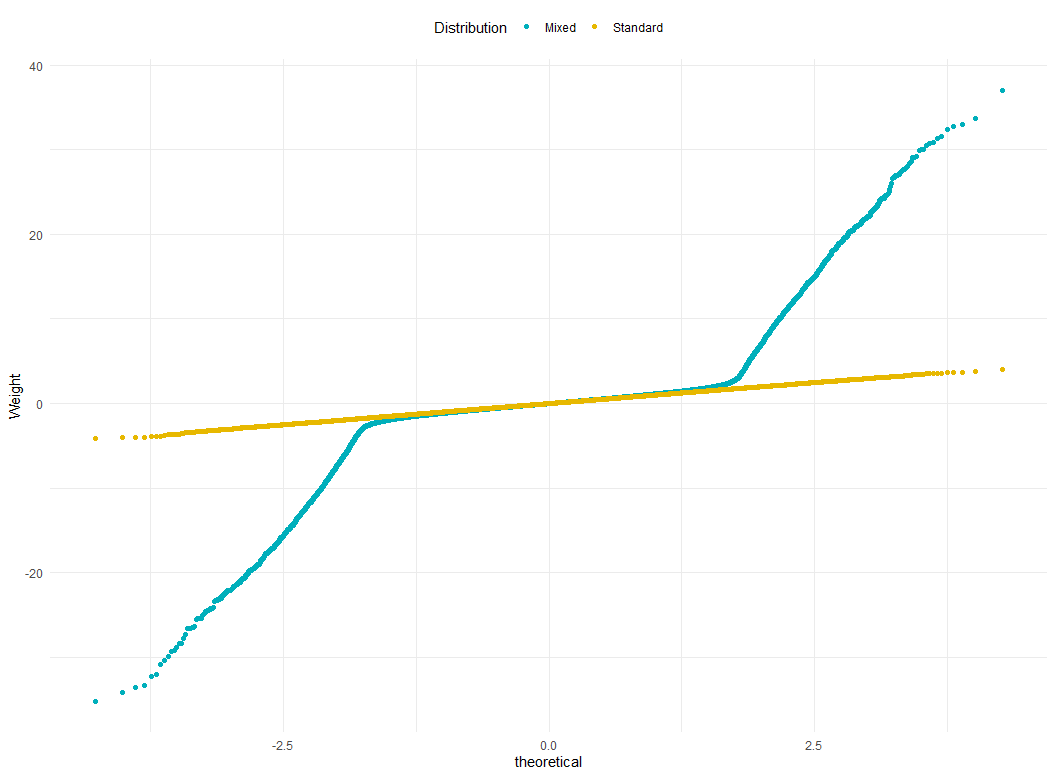
\includegraphics[width=0.8\textwidth,height=\textheight]{Images/Wilcox-2-QQ-Plot.jpg}
\caption{Q-Q-Plot of standard vs.~mixed normal (later is also reffered to as contaminated normal)}
\end{figure}

\subsection*{Issues with normality}\label{issues-with-normality}
\addcontentsline{toc}{subsection}{Issues with normality}

There are three issues related to normality:

\begin{enumerate}
\def\labelenumi{\arabic{enumi}.}
\tightlist
\item
  normality of residuals (\(\varepsilon_i\))
\item
  Normal distribution of test statistics
\item
  Confidence intervals
\end{enumerate}

\subsubsection*{Residuals}\label{residuals}
\addcontentsline{toc}{subsubsection}{Residuals}

The well known (simple) regression model in its mathematical form is defined as:

\begin{equation}
  Y_i = b_0 + X_i \cdot b_1 + \varepsilon_i
\end{equation}

Each case (\(i\)) of data (\(X_i\)) has a residual \(\varepsilon_i\), which is the difference between the predicted and observed values of the outcome. If you inspected a histogram of these residuals for all cases, you would hope to see a normal distribution centered around 0, i.e.~\(\bar{\varepsilon}_i = 0\).

A mean residual of \(\bar{\varepsilon}_i = 0\) means that the model (on average) correctly predicts the outcome value. In other words, if the residual is zero (or close to it) for most cases, then the error in prediction is zero (or close to it) for most cases.

If the model fits well, we might also expect that very extreme over-, or underestimations occur rarely. A well fitting model then would yield residuals that, like a normal distribution, are most frequent around zero and very infrequent at extreme values. This description explains what we mean by normality of residuals.

\begin{quote}
It also gives an idea of what it means if the normality of residuals is not given!
\end{quote}

\subsubsection*{Test statistics}\label{test-statistics}
\addcontentsline{toc}{subsubsection}{Test statistics}

The \(p\)-values associated with the parameter estimates of the model are based on the assumption that the test statistic associated with them follows a normal distribution (or some variant of it such as the \(t\)-distribution).

Essentially, to test the hypothesis that the parameter estimate (\(\bar{x}, r, \hat{b}_k\), etc.) is not equal to 0 (= \(H_1\)) it is necessary to assume a particular shape for the null distribution of the test statistic (i.e., normal).

If the sampling distribution of the test statistic turns out not to be the assumed shape (i.e.~normal) then the resulting \(p\)-values will be incorrect.

\begin{quote}
As a reminder: the \(p\)-value tells us about the probability to observe such data as our sample, IF the Null-Hyothesis (\(H_0\)) is True, i.e.~\(p(D|H_0)\)! For the \(H_0\) we (often) assume a normal distribution (or a deriviate of a normal, such as \(\chi^2, F, t\)).
\end{quote}

\subsubsection*{Confidence intervalls}\label{confidence-intervalls}
\addcontentsline{toc}{subsubsection}{Confidence intervalls}

The bounds of confidence intervals for parameter estimates are constructed by adding or subtracting from the estimate the associated standard error multiplied by the quantile of a null distribution associated with the probability level assigned to the interval.

\[\begin{array}{ccc}
  CI_{Mean} & = & \bar{x} \pm SE_{Mean} \cdot t_{crit}\\
  CI_{Corr} & = & r \pm SE_{Corr} \cdot t_{crit}\\
  CI_{Coef} & = & \hat{b}_k \pm SE_{Coeff} \cdot t_{crit} \\
  CI_{...}  & = & \cdots \pm SE_{...} \cdot t_{crit}
\end{array}\]

For tests of parameters in the linear model, the null distribution is assumed to be normal. It is an example of a general strategy in inferential statistics to convert an estimator, such as the mean, into a standardized statistic (z) that is asymptotically standard normal. The general issue is one of determining under what circumstances assuming normality gives a reasonably accurate result.

\section*{Myth and misconceptions about robustness}\label{myth-and-misconceptions-about-robustness}
\addcontentsline{toc}{section}{Myth and misconceptions about robustness}

\begin{quote}
A common claim, based on the \emph{central limit theorem}, is that with sample sizes greater than 30 the parameter estimate will have a normal sampling distribution. The implication being that if our sample is large we need not worry about checking normality to know that confidence intervals and p-values for a parameter estimate will be accurate. In which case, we can effectively ignore normality in all but quite exceptional cases of fitting a linear model.
\end{quote}

However, two things were missed when arriving at this conclusion:

\begin{enumerate}
\def\labelenumi{\arabic{enumi}.}
\tightlist
\item
  the conclusion is based on work using very light-tailed distributions.
\end{enumerate}

\begin{figure}
\centering
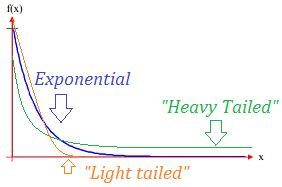
\includegraphics[width=0.4\textwidth,height=\textheight]{Images/LightHeavyDistribution.JPG}
\caption{Tails of a distribution}
\end{figure}

\begin{enumerate}
\def\labelenumi{\arabic{enumi}.}
\setcounter{enumi}{1}
\tightlist
\item
  the assumption that Student's \(T\) performs well if the sample mean has (to a close approximation) a normal distribution turns out to be incorrect under general conditions (Wilcox, 2016, 2017).
\end{enumerate}

\subsection*{Are GLM's robust?}\label{are-glms-robust}
\addcontentsline{toc}{subsection}{Are GLM's robust?}

Recent investigations revealed that differences in:

\begin{itemize}
\tightlist
\item
  \emph{skewness}
\item
  \emph{non-normality} and
\item
  \emph{heteroscedasticity}
\end{itemize}

interact in complicated ways that impact power (Wilcox, 2017). It was believed that as \emph{kurtosis} increases, the Type I error rate decreases and quickly drops below its nominal \(\alpha = .050\) level, and consequently power decreases (Glass et al., 1972).

\begin{quote}
This conclusion is correct only if \emph{distributions have the same amount of skewness}, because in this situation the difference between variables will have a \emph{symmetric distribution}.
\end{quote}

\emph{Unequal variances} (violations of \emph{homoscedasticity}), have relatively little influence when:

\begin{itemize}
\tightlist
\item
  group sizes are equal and
\item
  the normality assumption is true
\end{itemize}

But when group sizes are unequal F varies as a function of whether the largest group has the smallest variance or vice versa (see Field, Miles, \& Field, 2012, for a review).

\begin{quote}
When normality cannot be assumed equal group sizes do not save F from violations of homoscedasticity (Wilcox, 2010, 2016, 2017).
\end{quote}

\subsection*{Validity of central limit theorem}\label{validity-of-central-limit-theorem}
\addcontentsline{toc}{subsection}{Validity of central limit theorem}

When distributions are symmetric and have light tails the sampling distribution of means is approximately normal using samples of only \(N \approx 20\).

When distributions are asymmetric (skewed), even light-tailed distributions can require sample sizes of \(N \approx 200\) (e.g.~for one-sample t-tests).

Heteroscedasticity, makes matters worse. When distributions have heavy tails samples need to be much larger (up to \(N \approx 160\)) before the sampling distribution is normal (Wilcox, 2010).

\begin{quote}
As such, researchers can be lured into a false sense of security that they can assume normality of the sampling distribution because of the central limit theorem.
\end{quote}

\part*{PART II: Robust Methods}\label{part-part-ii-robust-methods}
\addcontentsline{toc}{part}{PART II: Robust Methods}

\section*{Definition of Robust}\label{definition-of-robust}
\addcontentsline{toc}{section}{Definition of Robust}

If we look up Wikipedia we find the following description of \href{https://en.wikipedia.org/wiki/Robust_statistics}{Robust Statistic}:

\emph{Robust statistics} are statistics with good performance for data drawn from a wide range of probability distributions, especially for distributions that are not normal.

\emph{Robust statistical methods} have been developed for many common problems, such as estimating location, scale, and regression parameters. One motivation is to produce statistical methods that are not unduly affected by outliers.

Another motivation is to provide methods with good performance when there are small departures from parametric distribution. For example, robust methods work well for mixtures of two normal distributions with different standard-deviations; under this model, non-robust methods like a t-test work poorly. Another definition of robust measures frequently used is:

\begin{quote}
Measures that characterize a distribution (such as location and scale) are said to be \emph{robust}, if slight changes in a distribution have a relatively small effect on their value (\citeproc{ref-Wilcox.2012}{Wilcox 2012}) (page 23).
\end{quote}

The mathematical foundation of robust methods (dealing with quantitative, qualitative and infnitesimal robustness of parameters) makes no assumptions regarding the functional form of the probability distribution.

The basic trick is to view parameters as functionals; expressions for the standard error follow from the influence function. Robust inferential methods are available that perform well with relatively small sample sizes, even in situations where classic methods based on means and variances perform poorly with relatively large sample sizes. Modern robust methods have the potential of substantially increasing power even under slight departures from normality. And perhaps more importantly, they can provide a deeper, more accurate and more nuanced understanding of data compared to classic techniques based on means.

\section*{Solutions to violated assumptions}\label{solutions-to-violated-assumptions}
\addcontentsline{toc}{section}{Solutions to violated assumptions}

The consequences of normality deviations such as:

\begin{itemize}
\tightlist
\item
  skewed distributions
\item
  data with outliers, or
\item
  heavy-tailed distributions
\end{itemize}

can influence the results of any classical (i.e.~parametric) statistical analysis quite substantially. Seen from a purely descriptive angle, it is trivial that the mean can be heavily affected by outliers or highly skewed distributional shapes.

\subsection*{Alternative estimators}\label{alternative-estimators}
\addcontentsline{toc}{subsection}{Alternative estimators}

Computing the mean on ``ugly'' data is just not a good location measure to characterize the sample. In this case one strategy is to use more robust measures such as the \emph{median} or the \emph{trimmed mean}, \emph{winsorized mean}, etc. and perform tests based on the corresponding sampling distribution of such robust measures.

It is quite common in experimental psychopathology research to do manual trims of the data based on outlier detection techniques (e.g., standard deviation based trims\footnote{ e.g.~Ratcliff (1993), with reaction time data to use standard deviation based trims such as excluding scores greater than 2.5 standard deviations from the mean. Be aware that this approach is flawed because both the mean and standard deviation are highly influenced by outliers (whether overt ones, or covert ones such as in a mixed normal distribution!} or idiosyncratic deletion).

Other popular alternatives are the M-estimators. They determine whether a score is an outlier empirically and if it is, adjustments are made for it. The adjustment could be to completely ignore the observation or to down-weight it. Obvious advantages of M-estimators are that you can:

\begin{enumerate}
\def\labelenumi{\arabic{enumi}.}
\tightlist
\item
  down-weight rather than exclude observations.
\item
  avoid over- or under-trimming your data.
\item
  perform non-symmetric trimming (\citeproc{ref-Wilcox.2012}{Wilcox 2012})
\end{enumerate}

When assumptions (independent, homoscedastic and normally-distributed errors) are not met, the ML estimator will yield different results to the OLS. The ML estimator is a lot more versatile than OLS and tends to be the default for more complex variants of the linear model (such as multilevel models, models with latent variables etc.).

\subsection*{Transformation of data}\label{transformation-of-data}
\addcontentsline{toc}{subsection}{Transformation of data}

Another strategy to deal with such violations (especially with skewed data) is to apply \href{https://en.wikipedia.org/wiki/Data_transformation_(statistics)}{transformations}
such as the \emph{logarithm} or more sophisticated \href{https://de.wikipedia.org/wiki/Box-Cox-Transformation}{Box-Cox transformations}. However, before working with transformed data, the following points should be considered (also see \citeproc{ref-Wilcox.2012}{Wilcox 2012}):

\begin{enumerate}
\def\labelenumi{\arabic{enumi}.}
\tightlist
\item
  transformations seldom improve the validity of probability statements.
\item
  transforming changes the hypothesis being tested (log transformed means compare geometric, rather than arithmetic means).
\item
  transforming the data also transforms the construct that it measures, so interpretation might become difficult.
\item
  the consequences of applying the `wrong' transformation must be less severe than the consequences of analyzing the untransformed scores.
\item
  heavy tails matter more than skew, so a transformation would need to address (and not make worse) any problems related to tail weight!
\item
  distributions often remain skewed after transformation.
\item
  transformations generally do not deal effectively with (real) outliers.
\end{enumerate}

\subsection*{Nonparametric tests}\label{nonparametric-tests}
\addcontentsline{toc}{subsection}{Nonparametric tests}

Another option is to switch into the nonparametric testing world (\citeproc{ref-Brunner.2002}{Brunner E. 2002}). Prominent examples for classical nonparametric tests taught in most introductory statistics class are:

\begin{itemize}
\tightlist
\item
  Mann-Whitney U-test (Mann and Whitney, 1947)
\item
  Wilcoxon signed-rank and rank-sum test (Wilcoxon, 1945)
\item
  Kruskal-Wallis ANOVA (Kruskal and Wallis 1952)
\item
  Friedmann ANOVA (Friedmann, 1937)
\end{itemize}

\subsection*{Robust methods}\label{robust-methods}
\addcontentsline{toc}{subsection}{Robust methods}

Developments of robust methods can be traced back to the 1960's with publications by Tukey (1960), Huber (1964), and Hampel (1968).

Modern robust methods have the potential of:

\begin{itemize}
\tightlist
\item
  substantially increasing power even under slight departures from normality.
\item
  can provide a deeper, more accurate and more nuanced understanding of data
\end{itemize}

compared to classic techniques based on means.

\subsection*{Adjusting the standard errors}\label{adjusting-the-standard-errors}
\addcontentsline{toc}{subsection}{Adjusting the standard errors}

There are ways to adjust standard errors to be robust in the presence of heteroscedasticity. One is known as the \emph{Eiker-White-Huber} heteroscedasticity-consistent stranded errors. The resulting robust standard errors can be used to compute confidence intervals, test-statistics (and associated p-values) that are robust to heteroscedasticity.

Another way to deal with bias in standard errors and (confidence intervals) is to estimate them empirically. The \emph{Bootstrap} is a flexible and general empirical method to find standard errors and confidence intervals for any statistic that is usually more accurate than traditional approaches. As with heteroscedasticityconsistent standard errors, bootstrap standard errors (and associated test statistics and p-values) and confidence intervals should be robust to violations of the assumptions.

\section*{Selected Robust measures of location}\label{selected-robust-measures-of-location}
\addcontentsline{toc}{section}{Selected Robust measures of location}

Measures of location are core elements of robust methods. Such measurese are:

\begin{itemize}
\tightlist
\item
  Trimmend mean
\item
  Winsorized mean
\item
  Huber M-estimator
\end{itemize}

\subsection*{Trimmed mean}\label{trimmed-mean}
\addcontentsline{toc}{subsection}{Trimmed mean}

The trimmed mean discards a certain percentage at both ends of the distribution. For instance, a 20\% trimmed mean cuts off 20\% at the low end and 20\% the high end. In R, a trimmed mean can be computed via the basic mean function by setting the trim argument accordingly. The following code also shows in which way the trimmed mean is calculated when the argument \texttt{trim} of the mean function is set to a value \(> 0\).

\begin{Shaded}
\begin{Highlighting}[]
  \FunctionTok{set.seed}\NormalTok{(}\DecValTok{423}\NormalTok{)}
\NormalTok{  N       }\OtherTok{\textless{}{-}} \DecValTok{20} \CommentTok{\# length of sample}
\NormalTok{  M       }\OtherTok{\textless{}{-}} \DecValTok{100} \CommentTok{\# Mean of sample}
\NormalTok{  SD      }\OtherTok{\textless{}{-}} \DecValTok{15}  \CommentTok{\# standard deviation of sample}
\NormalTok{  TF      }\OtherTok{\textless{}{-}} \FloatTok{0.1} \CommentTok{\# Trim{-}Faktor}
  \CommentTok{\#=== Generate Data ===}
\NormalTok{  IQ      }\OtherTok{\textless{}{-}} \FunctionTok{rnorm}\NormalTok{(N, }\AttributeTok{mean =}\NormalTok{ M, }\AttributeTok{sd =}\NormalTok{ SD)}
\NormalTok{  IQ[N]   }\OtherTok{\textless{}{-}} \DecValTok{1240} \CommentTok{\# introduce outlier}
  \FunctionTok{set.seed}\NormalTok{(}\DecValTok{2384}\NormalTok{)}
  \CommentTok{\#=== Manual trim ===}
  \CommentTok{\# IQ\_Red  \textless{}{-} sort(na.omit(IQ)) \# remove NA\textquotesingle{}s and sort}
\NormalTok{  IQ\_Sort }\OtherTok{\textless{}{-}} \FunctionTok{sort}\NormalTok{(IQ) }\CommentTok{\# sort Vector}
\NormalTok{  RedLgth }\OtherTok{\textless{}{-}}\NormalTok{ N}\SpecialCharTok{*}\NormalTok{TF}
\NormalTok{  TInd    }\OtherTok{\textless{}{-}}\NormalTok{ (RedLgth}\SpecialCharTok{+}\DecValTok{1}\NormalTok{)}\SpecialCharTok{:}\NormalTok{(N }\SpecialCharTok{{-}}\NormalTok{ RedLgth)}
\NormalTok{  IQ\_Trim }\OtherTok{\textless{}{-}}\NormalTok{ IQ\_Sort[TInd]}
  \CommentTok{\#=== Means ===}
\NormalTok{  M1      }\OtherTok{\textless{}{-}} \FunctionTok{round}\NormalTok{(}\FunctionTok{mean}\NormalTok{(IQ, }\AttributeTok{na.rm =}\NormalTok{ T), }\DecValTok{3}\NormalTok{)}
\NormalTok{  M2      }\OtherTok{\textless{}{-}} \FunctionTok{round}\NormalTok{(}\FunctionTok{mean}\NormalTok{(IQ, }\AttributeTok{na.rm =}\NormalTok{ T, }\AttributeTok{trim =}\NormalTok{ TF), }\DecValTok{3}\NormalTok{)}
\NormalTok{  M3      }\OtherTok{\textless{}{-}} \FunctionTok{round}\NormalTok{(}\FunctionTok{mean}\NormalTok{(IQ\_Trim, }\AttributeTok{na.rm =}\NormalTok{ T), }\DecValTok{3}\NormalTok{)}
\NormalTok{  Means   }\OtherTok{\textless{}{-}} \FunctionTok{data.frame}\NormalTok{(}\AttributeTok{Mean =}\NormalTok{ M1, }\AttributeTok{T\_Mean =}\NormalTok{ M2, }\AttributeTok{Man\_T\_Mean =}\NormalTok{ M3)}
\NormalTok{  knitr}\SpecialCharTok{::}\FunctionTok{kable}\NormalTok{(Means, }\AttributeTok{booktabs =} \ConstantTok{TRUE}\NormalTok{, }\AttributeTok{caption =} \StringTok{\textquotesingle{}mean vs. trimmed mean\textquotesingle{}}\NormalTok{)}
\end{Highlighting}
\end{Shaded}

\begin{table}

\caption{\label{tab:TrimmedMean}mean vs. trimmed mean}
\centering
\begin{tabular}[t]{rrr}
\toprule
Mean & T\_Mean & Man\_T\_Mean\\
\midrule
159.085 & 103.143 & 103.143\\
\bottomrule
\end{tabular}
\end{table}

\begin{Shaded}
\begin{Highlighting}[]
  \CommentTok{\#=== SDs ===}
\NormalTok{  SD1     }\OtherTok{\textless{}{-}} \FunctionTok{round}\NormalTok{(}\FunctionTok{sd}\NormalTok{(IQ) }\SpecialCharTok{/} \FunctionTok{sqrt}\NormalTok{(}\FunctionTok{length}\NormalTok{(IQ)), }\DecValTok{3}\NormalTok{)      }\CommentTok{\# standard error}
\NormalTok{  SD2     }\OtherTok{\textless{}{-}} \FunctionTok{round}\NormalTok{(}\FunctionTok{sd}\NormalTok{(IQ\_Trim)}\SpecialCharTok{/} \FunctionTok{sqrt}\NormalTok{(}\FunctionTok{length}\NormalTok{(IQ\_Trim)), }\DecValTok{3}\NormalTok{) }\CommentTok{\# standard error trimmed}
\NormalTok{  SD3     }\OtherTok{\textless{}{-}} \FunctionTok{round}\NormalTok{(}\FunctionTok{trimse}\NormalTok{(IQ, }\AttributeTok{tr =}\NormalTok{ TF), }\DecValTok{3}\NormalTok{)      }\CommentTok{\# standard error from WRS2}
\NormalTok{  StdDevs }\OtherTok{\textless{}{-}} \FunctionTok{data.frame}\NormalTok{(}\AttributeTok{SD =}\NormalTok{ SD1, }\AttributeTok{T\_SD =}\NormalTok{ SD2, }\AttributeTok{WRS2\_SD =}\NormalTok{ SD3)}
\NormalTok{  knitr}\SpecialCharTok{::}\FunctionTok{kable}\NormalTok{(StdDevs, }\AttributeTok{booktabs =} \ConstantTok{TRUE}\NormalTok{, }\AttributeTok{caption =} \StringTok{\textquotesingle{}Standard deviations\textquotesingle{}}\NormalTok{)}
\end{Highlighting}
\end{Shaded}

\begin{table}

\caption{\label{tab:TrimmedMean}Standard deviations}
\centering
\begin{tabular}[t]{rrr}
\toprule
SD & T\_SD & WRS2\_SD\\
\midrule
56.988 & 3.292 & 4.295\\
\bottomrule
\end{tabular}
\end{table}

Note that if the trimming portion is set to \(\gamma = 0.5\), the trimmed mean \(\bar{x}_t\) results in the \emph{median} \(\tilde{x}\) (which by itself \emph{reflects another robust location measure}).

\subsection*{Winsorized mean}\label{winsorized-mean}
\addcontentsline{toc}{subsection}{Winsorized mean}

A further robust location alternative to the mean is the \emph{Winsorized mean}.

\begin{quote}
The process of giving less weight to observations in the tails of the distribution and higher weight to the ones in the center is called \emph{Winsorizing}.
\end{quote}

Instead of computing the mean on the original distribution we compute the mean on the Winsorized distribution. Similar to the trimmed mean, the amount of Winsorizing (i.e., the \emph{Winsorizing level}) has to be choosen a priori. The \texttt{WRS2} function to compute Windsorized means is called \texttt{winmean}.

There is also a function supplied in the \texttt{DescTools} Package, the \texttt{DescTools::Winsorize()} function. The following code and output shows some examples of these estimators:

\begin{Shaded}
\begin{Highlighting}[]
  \CommentTok{\#=== Generate Data}
\NormalTok{  timevec }\OtherTok{\textless{}{-}} \FunctionTok{c}\NormalTok{(}\DecValTok{92}\NormalTok{, }\DecValTok{19}\NormalTok{, }\DecValTok{101}\NormalTok{, }\DecValTok{58}\NormalTok{, }\DecValTok{1053}\NormalTok{, }\DecValTok{91}\NormalTok{, }\DecValTok{26}\NormalTok{, }\DecValTok{78}\NormalTok{, }\DecValTok{10}\NormalTok{, }\DecValTok{13}\NormalTok{, }\SpecialCharTok{{-}}\DecValTok{40}\NormalTok{, }\DecValTok{101}\NormalTok{, }
               \DecValTok{86}\NormalTok{, }\DecValTok{85}\NormalTok{, }\DecValTok{15}\NormalTok{, }\DecValTok{89}\NormalTok{, }\DecValTok{89}\NormalTok{, }\DecValTok{28}\NormalTok{, }\SpecialCharTok{{-}}\DecValTok{5}\NormalTok{, }\DecValTok{41}\NormalTok{)}
  \CommentTok{\# timevec \textless{}{-} c( 77,  87,  88, 114, 151, 210, 219,  246, 253, 262, }
  \CommentTok{\#              296, 299, 306, 376, 428, 515, 666, 1310, 2611)}
\NormalTok{  timevec }\OtherTok{\textless{}{-}} \FunctionTok{sort}\NormalTok{(timevec)}
  \CommentTok{\#=== Trimmed Mean and SE}
\NormalTok{  TM      }\OtherTok{\textless{}{-}} \FunctionTok{mean}\NormalTok{(timevec, }\AttributeTok{trim =}\NormalTok{ TF) }\CommentTok{\# calculate the trimmed mean of the time vector}
\NormalTok{  TSE     }\OtherTok{\textless{}{-}} \FunctionTok{trimse}\NormalTok{(timevec, }\AttributeTok{tr =}\NormalTok{ TF) }\CommentTok{\#calculate the trimmed mean of the time vector}
  \CommentTok{\#=== Winsorized Mean an SE, Median and SE of Median}
\NormalTok{  WinS\_Mean }\OtherTok{\textless{}{-}} \FunctionTok{winmean}\NormalTok{(timevec, }\AttributeTok{tr =}\NormalTok{ TF, }\AttributeTok{na.rm =} \ConstantTok{FALSE}\NormalTok{) }\CommentTok{\# winsorized mean}
\NormalTok{  WinS\_SE   }\OtherTok{\textless{}{-}} \FunctionTok{winse}\NormalTok{(timevec, }\AttributeTok{tr =}\NormalTok{ TF) }\CommentTok{\# winsorized mean}
\NormalTok{  Med       }\OtherTok{\textless{}{-}} \FunctionTok{median}\NormalTok{(timevec) }\CommentTok{\# winsorized mean}
\NormalTok{  Med\_SE    }\OtherTok{\textless{}{-}} \FunctionTok{msmedse}\NormalTok{(timevec) }\CommentTok{\# winsorized mean}
\NormalTok{  tv\_DT     }\OtherTok{\textless{}{-}}\NormalTok{ DescTools}\SpecialCharTok{::}\FunctionTok{Winsorize}\NormalTok{(timevec, }
                                    \AttributeTok{val =} \FunctionTok{quantile}\NormalTok{(timevec, }
                                                   \AttributeTok{probs =} \FunctionTok{c}\NormalTok{(TF, }\DecValTok{1}\SpecialCharTok{{-}}\NormalTok{TF),}
                                    \AttributeTok{na.rm =} \ConstantTok{FALSE}\NormalTok{))}
\NormalTok{  M\_DT      }\OtherTok{\textless{}{-}} \FunctionTok{mean}\NormalTok{(tv\_DT)}
  \CommentTok{\#=== manually winsorized}
\NormalTok{  QTV              }\OtherTok{\textless{}{-}} \FunctionTok{quantile}\NormalTok{(timevec, }\AttributeTok{probs =} \FunctionTok{c}\NormalTok{(TF, }\DecValTok{1}\SpecialCharTok{{-}}\NormalTok{TF))}
\NormalTok{  QTIndUG          }\OtherTok{\textless{}{-}}\NormalTok{ timevec }\SpecialCharTok{\textless{}=}\NormalTok{ QTV[}\DecValTok{1}\NormalTok{]}
\NormalTok{  QTIndOG          }\OtherTok{\textless{}{-}}\NormalTok{ timevec }\SpecialCharTok{\textgreater{}=}\NormalTok{ QTV[}\DecValTok{2}\NormalTok{]}
\NormalTok{  timevec[QTIndUG] }\OtherTok{\textless{}{-}}\NormalTok{ QTV[}\DecValTok{1}\NormalTok{]}
\NormalTok{  timevec[QTIndOG] }\OtherTok{\textless{}{-}}\NormalTok{ QTV[}\DecValTok{2}\NormalTok{]}
\NormalTok{  ManMeanWS        }\OtherTok{\textless{}{-}} \FunctionTok{mean}\NormalTok{(timevec)}
\end{Highlighting}
\end{Shaded}

Note that winsorizing is not equivalent to simply excluding (trimming) data, but is a method of censoring data. Thus a winsorized mean is not the same as a truncated mean (cf.~\href{https://en.wikipedia.org/wiki/Winsorizing}{Winsorizing, Wikipedia}).

\begin{itemize}
\tightlist
\item
  the 10\% trimmed mean is the average of the 5th to 95th percentile of the data
\item
  the 90\% winsorized mean sets the bottom 5\% to the 5th percentile, the top 5\% to the 95th percentile, and then averages the data.
\end{itemize}

\subsubsection*{Winsorization Round-Up}\label{winsorization-round-up}
\addcontentsline{toc}{subsubsection}{Winsorization Round-Up}

Following round-up is taken from this \href{https://blogs.sas.com/content/iml/2017/02/08/winsorization-good-bad-and-ugly.html}{SAS-blog}:

\textbf{The good:}

\begin{itemize}
\tightlist
\item
  The purpose of Winsorization is to ``robustify'' classical statistics by reducing the impact of extreme observations.
\item
  If you compare a Winsorized statistic with classical statistic, you can identify variables that might contain contaminated data or are long-tailed and require special handling in models.
\end{itemize}

\textbf{The ugly:}

Modifying the data is a draconian measure. In his book (\citeproc{ref-Tukey.1960}{Tukey 2009}), he says:

When statisticians encounter a few extreme values in data, we are likely to think of them as \emph{strays}, \emph{wild shots} and to focus our attention on how normally distributed the rest of the distribution appears to be. One who does this commits two oversights:

\begin{itemize}
\tightlist
\item
  forgetting Winsor's principle that \emph{all distributions are normal in the middle}, and
\item
  forgetting that the distribution relevant to statistical practice is that of the values actually provided and not of the values which ought to have been provided.
\end{itemize}

Concluding a bit further on:

\begin{quote}
Sets of observations which have been \emph{de-tailed} by \emph{over-vigorous} use of a rule for rejecting outliers are inappropriate, since they are not samples.
\end{quote}

\subsection*{M-estimators}\label{m-estimators}
\addcontentsline{toc}{subsection}{M-estimators}

A general family of robust location measures are so called \(M\)-estimators (the \(M\) stands for \textbf{M}aximum Likelihood-type''). They are based on a loss function to be minimized. Huber (1981) proposed a function (cf. \citeproc{ref-Wilcox.2012}{Wilcox 2012}) in which a \emph{bending constant \textbf{K} } increases sensitivity to the tails of the distribution. The estimation of M-estimators is performed iteratively and implemented in the \texttt{mest()} function.

\begin{Shaded}
\begin{Highlighting}[]
\NormalTok{  MWHub }\OtherTok{\textless{}{-}} \FunctionTok{mest}\NormalTok{(timevec, }\AttributeTok{bend =} \FloatTok{1.28}\NormalTok{, }\AttributeTok{na.rm =} \ConstantTok{FALSE}\NormalTok{) }\CommentTok{\# Huber{-}estimator}
\NormalTok{  SEHub }\OtherTok{\textless{}{-}} \FunctionTok{mestse}\NormalTok{(timevec)                           }\CommentTok{\# Huber{-}estimator for SE}
\end{Highlighting}
\end{Shaded}

\section*{Measures of Scale}\label{measures-of-scale}
\addcontentsline{toc}{section}{Measures of Scale}

There are several robust measure of scales, of which we will only name a few, without getting into the mathematical details of their properties. Currently there are two general approaches to measuring scale that are of importance:

\begin{enumerate}
\def\labelenumi{\arabic{enumi}.}
\tightlist
\item
  \href{https://en.wikipedia.org/wiki/L-estimator}{L-measures}: is an estimator which is a linear combination of order statistics\footnote{together with rank statistics, order statistics are among the most fundamental tools in non-parametric statistics and inference. Examples of order statistics are maximum, minimum, range, quantiles, median, etc.} of the measurements (which is also called an L-statistic). This can be as little as a single point, as in the median (of an odd number of values), or as many as all points, as in the mean. The main benefits of L-estimators are that they are often extremely simple, and \emph{robust}.
\item
  \href{https://en.wikipedia.org/wiki/M-estimator}{M-measures}: proposedby Huber (1964) these measures are a generalization of the maximum likelihood estimations. The \(M\) stands for \emph{Maximum likelihood type}. M-measures can be constructed for location parameters and scale parameters in univariate and multivariate settings, as well as being used in robust regression.
\end{enumerate}

Different measures of scale used frequently are:

\begin{enumerate}
\def\labelenumi{\arabic{enumi}.}
\tightlist
\item
  Mean Deviation from the Mean
\item
  Mean Deviation from the Median
\item
  Median Absolute Deviation
\item
  q-Quantile Range
\item
  Winsorized Variance
\end{enumerate}

Some of these measures will be used and discussed in the next chapter. For further details to their definition and properties refer to (page36 \citeproc{ref-Wilcox.2012}{Wilcox 2012}).

\part*{PART III: R-Examples}\label{part-part-iii-r-examples}
\addcontentsline{toc}{part}{PART III: R-Examples}

\section*{R-Packages}\label{r-packages}
\addcontentsline{toc}{section}{R-Packages}

We will use the \href{https://cran.r-project.org/web/packages/WRS2/WRS2.pdf}{WRS2} (Mair, Schoenbrodt, \& Wilcox, 2017), \href{https://cran.r-project.org/web/packages/robustbase/robustbase.pdf}{robustbase} (Rousseeuw et al., 2015), and \href{https://cran.r-project.org/web/packages/DescTools/DescTools.pdf}{DescTools} packages to access functions for some selected robust tests.

Furthermore, packages such as \href{https://cran.r-project.org/web/packages/lme4/lme4.pdf}{lme4} (Bates, Maechler, Bolker, \& Walker, 2015) and \href{https://cran.r-project.org/web/packages/robustlmm/robustlmm.pdf}{robustlmm} (Manuel Koller, 2016) for the multilevel model, and \href{https://cran.r-project.org/web/packages/lavaan/lavaan.pdf}{lavaan} (Rosseel, 2012) for the latent growth model will be used in the course of this workshop.

To access these packages, paste and copy the following code:

\begin{Shaded}
\begin{Highlighting}[]
  \FunctionTok{rm}\NormalTok{(}\AttributeTok{list =} \FunctionTok{ls}\NormalTok{())}
  \FunctionTok{graphics.off}\NormalTok{()}
  \FunctionTok{options}\NormalTok{(}\AttributeTok{digits =} \DecValTok{2}\NormalTok{)}
  \ControlFlowTok{if}\NormalTok{ (}\SpecialCharTok{!}\FunctionTok{require}\NormalTok{(}\StringTok{"pacman"}\NormalTok{)) }\FunctionTok{install.packages}\NormalTok{(}\StringTok{"pacman"}\NormalTok{)}
\NormalTok{  pacman}\SpecialCharTok{::}\FunctionTok{p\_load}\NormalTok{(corrplot, corrr,}
\NormalTok{                 DescTools, dplyr,}
\NormalTok{                 ggplot2, ggridges, ggpubr,}
\NormalTok{                 knitr,}
\NormalTok{                 lavaan, lme4, }
\NormalTok{                 nlme, }
\NormalTok{                 pander,}
\NormalTok{                 readr, reshape, robustlmm, robustbase, rstatix,}
\NormalTok{                 tidyverse,}
\NormalTok{                 WRS2)}
  
    \DocumentationTok{\#\#\#\#\#\#\#\#\#\#\#\#\#\#\#\#\#\#\#\#\#\#\#\#\#\#\#\#\#\#\#\#\#\#\#\#\#\#\#\#\#\#\#\#\#\#\#}
\end{Highlighting}
\end{Shaded}

\emph{Note to the \texttt{DescTools} package:} the author's intention was to create a toolbox, which facilitates many of the tasks in data analysis, consisting of calculating descriptive statistics, drawing graphical summaries and reporting the results. The package contains furthermore functions to produce documents using MS Word (or PowerPoint) and functions to import data from Excel. Many of the included functions can be found scattered in other packages and other sources written partly by Titans of R. Important for us, robust methods such as robust estimators such as HuberM, TukeyBiweight, Robust data standardization, robust range, Yuen-t-Test, JarqueBeraTest, etc. can be found in this package.

\emph{Note to the \texttt{tidyverse} package:} the tidyverse is an opinionated collection of R packages designed for data science. All packages share an underlying design philosophy, grammar, and data structures.

\subsection*{Other Packages in R}\label{other-packages-in-r}
\addcontentsline{toc}{subsection}{Other Packages in R}

R is pretty well endowed with all sorts of robust functions and packages. For an extended overview see the additional packages for robust statistics on \href{https://cran.r-project.org/web/views/Robust.html}{CRAN}. From this list we name just a few as examples for the manifold statistical application areas:

\begin{itemize}
\tightlist
\item
  robust regression functions:

  \begin{itemize}
  \tightlist
  \item
    \textbf{rlm} in \texttt{MASS}\\
  \item
    \textbf{lmrob} and \textbf{nlrob} in \texttt{robustbase}
  \end{itemize}
\item
  robust mixed-effects models - \texttt{robustlmm}
\item
  robust generalized additive models - \texttt{robustgam}
\item
  multivariate methods:

  \begin{itemize}
  \tightlist
  \item
    \texttt{rrcov} (robust multivariate variance-covariance estimation and robust principal components analysis (PCA))
  \item
    \texttt{FRB} includes bootstrap based approaches for multivariate regression, PCA and Hotelling tests
  \item
    \texttt{RSKC} functions for robust \(k\)-means clustering
  \item
    \texttt{robustDA} performs robust discriminant analysis.
  \end{itemize}
\end{itemize}

\section*{Two independent means}\label{two-independent-means}
\addcontentsline{toc}{section}{Two independent means}

The data \emph{fileKellyetalz.csv} (\citeproc{ref-Kelly.2010}{Kelly 2010}) can be downloaded from the Blackboard.The file contains the data from a survey that investigated whether verbal information or modelling were effective in reversing the effect of verbal threat information on children's fears of novel animals.

Children aged 6-8 years old were given threat information or no information about two novel Australian marsupials. Following this information, different groups received one of three \emph{interventions}:

\begin{enumerate}
\def\labelenumi{\arabic{enumi}.}
\tightlist
\item
  positive information about the threat animal
\item
  a positive modelling experience (an adult placing their hand in a box seemingly containing the threat animal)
\item
  no further experience.
\end{enumerate}

The children's \emph{fear} of the marsupials was measured using a self-report measure called the \textbf{F}ear \textbf{B}eliefs \textbf{Q}uestionnaire (\emph{FBQ}) or a \textbf{B}ehavioral \textbf{A}pproach \textbf{T}ask (\emph{BAT}) like that described before. In the paper, the authors test the specificity of the interventions by comparing their effects on the subjective (FBQ) and behavioural (BAT) components of the fear emotion. To do so, a single score was computed separately for the \emph{FBQ} and \emph{BAT} that represented the change from pre-to post-intervention for the threat animal relative to the control animal. These scores, therefore, represent the overall effect of the intervention on each measure. The scores were converted to z-scores separately for the \emph{FBQ} and \emph{BAT} so that they could be compared.

Note that because the interventions are expected to reduce fear, greater efficacy is shown up by more negative z-scores (i.e.~greater reductions in fear). This part of the study had a \emph{mixed design} with a between group manipulation of intervention:

\begin{itemize}
\tightlist
\item
  positive information
\item
  non-anxious modeling
\item
  no intervention
\end{itemize}

and a repeated measures manipulation of the type of measure (\emph{FBQ} or \emph{BAT}). The data file contains 4 variables:

\begin{enumerate}
\def\labelenumi{\arabic{enumi}.}
\tightlist
\item
  \texttt{id}: indicates the participant number;
\item
  \texttt{Intervention}: is a factor indicating whether the child received positive information, non-anxious modelling or no intervention,
\item
  \texttt{Measure}: indicates whether a score came from the \emph{FBQ} or \emph{BAT}
\item
  \texttt{z}: is the z-score associated with the measure.
\end{enumerate}

Note that \emph{FBQ} and \emph{BAT} scores are in long format (contrasted with the wide format with which SPSS users will be more familiar).

\begin{Shaded}
\begin{Highlighting}[]
    \CommentTok{\# Kelly et al. (2010)}
\NormalTok{    kellyz }\OtherTok{\textless{}{-}} \FunctionTok{read.csv}\NormalTok{(}\StringTok{"Daten/Kellyetalz.csv"}\NormalTok{)}
    \FunctionTok{pander}\NormalTok{(}\FunctionTok{head}\NormalTok{(kellyz, }\DecValTok{6}\NormalTok{), }\AttributeTok{digits =} \DecValTok{3}\NormalTok{)}
\end{Highlighting}
\end{Shaded}

\begin{longtable}[]{@{}
  >{\centering\arraybackslash}p{(\columnwidth - 6\tabcolsep) * \real{0.0972}}
  >{\centering\arraybackslash}p{(\columnwidth - 6\tabcolsep) * \real{0.3194}}
  >{\centering\arraybackslash}p{(\columnwidth - 6\tabcolsep) * \real{0.1389}}
  >{\centering\arraybackslash}p{(\columnwidth - 6\tabcolsep) * \real{0.1389}}@{}}
\toprule\noalign{}
\begin{minipage}[b]{\linewidth}\centering
id
\end{minipage} & \begin{minipage}[b]{\linewidth}\centering
Intervention
\end{minipage} & \begin{minipage}[b]{\linewidth}\centering
Measure
\end{minipage} & \begin{minipage}[b]{\linewidth}\centering
z
\end{minipage} \\
\midrule\noalign{}
\endhead
\bottomrule\noalign{}
\endlastfoot
egs1 & Positive Information & BAT & 0.204 \\
egs1 & Positive Information & FBQ & -0.614 \\
lrx2 & Positive Information & BAT & -0.0234 \\
lrx2 & Positive Information & FBQ & -1.49 \\
zej3 & Positive Information & BAT & -0.498 \\
zej3 & Positive Information & FBQ & -1.66 \\
\end{longtable}

\subsection*{Standard t-Test}\label{standard-t-test}
\addcontentsline{toc}{subsection}{Standard t-Test}

We are going to compare the \texttt{FBQ} z-scores in two conditions: \emph{positive information} vs.~\emph{No intervention}. To do this, we need to first select this subset of the data by executing these commands:

\begin{Shaded}
\begin{Highlighting}[]
\NormalTok{    posInfoFBQ }\OtherTok{\textless{}{-}} \FunctionTok{subset}\NormalTok{(kellyz, Intervention}\SpecialCharTok{!=} \StringTok{"Non{-}Anxious Modelling"} \SpecialCharTok{\&} 
\NormalTok{                           Measure }\SpecialCharTok{==} \StringTok{"FBQ"}\NormalTok{)}
\NormalTok{    posInfoFBQ}\SpecialCharTok{$}\NormalTok{Intervention }\OtherTok{\textless{}{-}} \FunctionTok{factor}\NormalTok{(posInfoFBQ}\SpecialCharTok{$}\NormalTok{Intervention)}
    \FunctionTok{pander}\NormalTok{(}\FunctionTok{head}\NormalTok{(posInfoFBQ[}\FunctionTok{order}\NormalTok{(posInfoFBQ}\SpecialCharTok{$}\NormalTok{id),], }\DecValTok{6}\NormalTok{))}
\end{Highlighting}
\end{Shaded}

\begin{longtable}[]{@{}
  >{\centering\arraybackslash}p{(\columnwidth - 8\tabcolsep) * \real{0.1389}}
  >{\centering\arraybackslash}p{(\columnwidth - 8\tabcolsep) * \real{0.1111}}
  >{\centering\arraybackslash}p{(\columnwidth - 8\tabcolsep) * \real{0.3194}}
  >{\centering\arraybackslash}p{(\columnwidth - 8\tabcolsep) * \real{0.1389}}
  >{\centering\arraybackslash}p{(\columnwidth - 8\tabcolsep) * \real{0.1389}}@{}}
\toprule\noalign{}
\begin{minipage}[b]{\linewidth}\centering
~
\end{minipage} & \begin{minipage}[b]{\linewidth}\centering
id
\end{minipage} & \begin{minipage}[b]{\linewidth}\centering
Intervention
\end{minipage} & \begin{minipage}[b]{\linewidth}\centering
Measure
\end{minipage} & \begin{minipage}[b]{\linewidth}\centering
z
\end{minipage} \\
\midrule\noalign{}
\endhead
\bottomrule\noalign{}
\endlastfoot
\textbf{60} & aqa30 & Positive Information & FBQ & -1.837 \\
\textbf{46} & asl23 & Positive Information & FBQ & 0.4333 \\
\textbf{8} & bcv4 & Positive Information & FBQ & -1.313 \\
\textbf{44} & bgi22 & Positive Information & FBQ & -0.5271 \\
\textbf{16} & czq8 & Positive Information & FBQ & 1.219 \\
\textbf{158} & dsl79 & No Intervention & FBQ & 0.5206 \\
\end{longtable}

The standard function \texttt{stats::t.test()} returns the \href{https://en.wikipedia.org/wiki/Welch\%27s_t-test}{Welch's} t-test statistic. It is also referred to as the \emph{unequal variances t-test}. It is an adaptation of Student's t-test and is more reliable when:

\begin{itemize}
\tightlist
\item
  the two samples have unequal variances and/or
\item
  unequal sample sizes.
\end{itemize}

\begin{Shaded}
\begin{Highlighting}[]
    \CommentTok{\# pander(t.test(z \textasciitilde{} Intervention, data = posInfoFBQ, var.equal = TRUE))}
    \FunctionTok{pander}\NormalTok{(}\FunctionTok{t.test}\NormalTok{(z }\SpecialCharTok{\textasciitilde{}}\NormalTok{ Intervention, }\AttributeTok{data =}\NormalTok{ posInfoFBQ))}
\end{Highlighting}
\end{Shaded}

\begin{longtable}[]{@{}
  >{\centering\arraybackslash}p{(\columnwidth - 6\tabcolsep) * \real{0.2361}}
  >{\centering\arraybackslash}p{(\columnwidth - 6\tabcolsep) * \real{0.1111}}
  >{\centering\arraybackslash}p{(\columnwidth - 6\tabcolsep) * \real{0.2500}}
  >{\centering\arraybackslash}p{(\columnwidth - 6\tabcolsep) * \real{0.3472}}@{}}
\caption{Welch Two Sample t-test: \texttt{z} by \texttt{Intervention} (continued below)}\tabularnewline
\toprule\noalign{}
\begin{minipage}[b]{\linewidth}\centering
Test statistic
\end{minipage} & \begin{minipage}[b]{\linewidth}\centering
df
\end{minipage} & \begin{minipage}[b]{\linewidth}\centering
P value
\end{minipage} & \begin{minipage}[b]{\linewidth}\centering
Alternative hypothesis
\end{minipage} \\
\midrule\noalign{}
\endfirsthead
\toprule\noalign{}
\begin{minipage}[b]{\linewidth}\centering
Test statistic
\end{minipage} & \begin{minipage}[b]{\linewidth}\centering
df
\end{minipage} & \begin{minipage}[b]{\linewidth}\centering
P value
\end{minipage} & \begin{minipage}[b]{\linewidth}\centering
Alternative hypothesis
\end{minipage} \\
\midrule\noalign{}
\endhead
\bottomrule\noalign{}
\endlastfoot
7.119 & 53.01 & 2.896e-09 * * * & two.sided \\
\end{longtable}

\begin{longtable}[]{@{}
  >{\centering\arraybackslash}p{(\columnwidth - 2\tabcolsep) * \real{0.4444}}
  >{\centering\arraybackslash}p{(\columnwidth - 2\tabcolsep) * \real{0.3472}}@{}}
\toprule\noalign{}
\begin{minipage}[b]{\linewidth}\centering
mean in group No Intervention
\end{minipage} & \begin{minipage}[b]{\linewidth}\centering
mean in group Positive
Information
\end{minipage} \\
\midrule\noalign{}
\endhead
\bottomrule\noalign{}
\endlastfoot
0.6553 & -0.7867 \\
\end{longtable}

\subsection*{Robust t-Test}\label{robust-t-test}
\addcontentsline{toc}{subsection}{Robust t-Test}

\begin{Shaded}
\begin{Highlighting}[]
    \FunctionTok{pander}\NormalTok{(}\FunctionTok{YuenTTest}\NormalTok{(z }\SpecialCharTok{\textasciitilde{}}\NormalTok{ Intervention, }\AttributeTok{data =}\NormalTok{ posInfoFBQ))}
\end{Highlighting}
\end{Shaded}

\begin{longtable}[]{@{}
  >{\centering\arraybackslash}p{(\columnwidth - 8\tabcolsep) * \real{0.2267}}
  >{\centering\arraybackslash}p{(\columnwidth - 8\tabcolsep) * \real{0.1067}}
  >{\centering\arraybackslash}p{(\columnwidth - 8\tabcolsep) * \real{0.0933}}
  >{\centering\arraybackslash}p{(\columnwidth - 8\tabcolsep) * \real{0.2400}}
  >{\centering\arraybackslash}p{(\columnwidth - 8\tabcolsep) * \real{0.3333}}@{}}
\caption{Yuen Two Sample t-test: \texttt{z} by \texttt{Intervention} (continued below)}\tabularnewline
\toprule\noalign{}
\begin{minipage}[b]{\linewidth}\centering
Test statistic
\end{minipage} & \begin{minipage}[b]{\linewidth}\centering
df
\end{minipage} & \begin{minipage}[b]{\linewidth}\centering
trim
\end{minipage} & \begin{minipage}[b]{\linewidth}\centering
P value
\end{minipage} & \begin{minipage}[b]{\linewidth}\centering
Alternative hypothesis
\end{minipage} \\
\midrule\noalign{}
\endfirsthead
\toprule\noalign{}
\begin{minipage}[b]{\linewidth}\centering
Test statistic
\end{minipage} & \begin{minipage}[b]{\linewidth}\centering
df
\end{minipage} & \begin{minipage}[b]{\linewidth}\centering
trim
\end{minipage} & \begin{minipage}[b]{\linewidth}\centering
P value
\end{minipage} & \begin{minipage}[b]{\linewidth}\centering
Alternative hypothesis
\end{minipage} \\
\midrule\noalign{}
\endhead
\bottomrule\noalign{}
\endlastfoot
6.244 & 28.84 & 0.2 & 8.371e-07 * * * & two.sided \\
\end{longtable}

\begin{longtable}[]{@{}
  >{\centering\arraybackslash}p{(\columnwidth - 2\tabcolsep) * \real{0.3750}}
  >{\centering\arraybackslash}p{(\columnwidth - 2\tabcolsep) * \real{0.4583}}@{}}
\toprule\noalign{}
\begin{minipage}[b]{\linewidth}\centering
trimmed mean in group No
Intervention
\end{minipage} & \begin{minipage}[b]{\linewidth}\centering
trimmed mean in group Positive
Information
\end{minipage} \\
\midrule\noalign{}
\endhead
\bottomrule\noalign{}
\endlastfoot
0.6245 & -0.7701 \\
\end{longtable}

\begin{Shaded}
\begin{Highlighting}[]
    \FunctionTok{pander}\NormalTok{(}\FunctionTok{yuenbt}\NormalTok{(z }\SpecialCharTok{\textasciitilde{}}\NormalTok{ Intervention, }\AttributeTok{data =}\NormalTok{ posInfoFBQ))}
\end{Highlighting}
\end{Shaded}

\begin{itemize}
\tightlist
\item
  \textbf{test}: \emph{6.071}
\item
  \textbf{conf.int}: \emph{0.8996} and \emph{1.89}
\item
  \textbf{p.value}: \emph{0}
\item
  \textbf{df}: \emph{NA}
\item
  \textbf{diff}: \emph{1.395}
\item
  \textbf{call}: \texttt{yuenbt(formula\ =\ z\ \textasciitilde{}\ Intervention,\ data\ =\ posInfoFBQ)}
\end{itemize}

\begin{Shaded}
\begin{Highlighting}[]
    \DocumentationTok{\#\#\#\#\#\#\#\#\#\#\#\#\#\#\#\#\#\#\#\#\#\#\#\#\#\#\#\#\#\#\#\#\#\#\#\#\#\#\#\#\#\#\#\#\#\#\#}
\end{Highlighting}
\end{Shaded}

We could report the robust test as a significant difference between trimmed mean \texttt{FBQ} z-scores in the positive information intervention compared to no intervention, \(M_{diff} = 1.39 \ [0.91, 1.88], \ Y_t = 6.07, \ p < 0.001\).

\section*{One-way ANOVA}\label{one-way-anova}
\addcontentsline{toc}{section}{One-way ANOVA}

As in the previous example, we create a new data frame that includes only the \texttt{FBQ} data:

\begin{Shaded}
\begin{Highlighting}[]
\NormalTok{    fbqOnly }\OtherTok{\textless{}{-}} \FunctionTok{subset}\NormalTok{(kellyz, Measure }\SpecialCharTok{==} \StringTok{"FBQ"}\NormalTok{)}
\end{Highlighting}
\end{Shaded}

\subsection*{Standard ANOVA}\label{standard-anova}
\addcontentsline{toc}{subsection}{Standard ANOVA}

The comparison of \texttt{FBQ} means across all three intervention groups can be done with an one-way independent ANOVA. We will compare the robust test to the classic linear model,
which can be obtained by executing:

\begin{Shaded}
\begin{Highlighting}[]
    \FunctionTok{pander}\NormalTok{(}\FunctionTok{summary}\NormalTok{(}\FunctionTok{aov}\NormalTok{(z }\SpecialCharTok{\textasciitilde{}}\NormalTok{ Intervention, }\AttributeTok{data =}\NormalTok{ fbqOnly)))}
\end{Highlighting}
\end{Shaded}

\begin{longtable}[]{@{}
  >{\centering\arraybackslash}p{(\columnwidth - 10\tabcolsep) * \real{0.2639}}
  >{\centering\arraybackslash}p{(\columnwidth - 10\tabcolsep) * \real{0.0833}}
  >{\centering\arraybackslash}p{(\columnwidth - 10\tabcolsep) * \real{0.1250}}
  >{\centering\arraybackslash}p{(\columnwidth - 10\tabcolsep) * \real{0.1389}}
  >{\centering\arraybackslash}p{(\columnwidth - 10\tabcolsep) * \real{0.1389}}
  >{\centering\arraybackslash}p{(\columnwidth - 10\tabcolsep) * \real{0.1667}}@{}}
\caption{Analysis of Variance Model}\tabularnewline
\toprule\noalign{}
\begin{minipage}[b]{\linewidth}\centering
~
\end{minipage} & \begin{minipage}[b]{\linewidth}\centering
Df
\end{minipage} & \begin{minipage}[b]{\linewidth}\centering
Sum Sq
\end{minipage} & \begin{minipage}[b]{\linewidth}\centering
Mean Sq
\end{minipage} & \begin{minipage}[b]{\linewidth}\centering
F value
\end{minipage} & \begin{minipage}[b]{\linewidth}\centering
Pr(\textgreater F)
\end{minipage} \\
\midrule\noalign{}
\endfirsthead
\toprule\noalign{}
\begin{minipage}[b]{\linewidth}\centering
~
\end{minipage} & \begin{minipage}[b]{\linewidth}\centering
Df
\end{minipage} & \begin{minipage}[b]{\linewidth}\centering
Sum Sq
\end{minipage} & \begin{minipage}[b]{\linewidth}\centering
Mean Sq
\end{minipage} & \begin{minipage}[b]{\linewidth}\centering
F value
\end{minipage} & \begin{minipage}[b]{\linewidth}\centering
Pr(\textgreater F)
\end{minipage} \\
\midrule\noalign{}
\endhead
\bottomrule\noalign{}
\endlastfoot
\textbf{Intervention} & 2 & 39.02 & 19.51 & 30.29 & 4.314e-11 \\
\textbf{Residuals} & 104 & 66.98 & 0.6441 & NA & NA \\
\end{longtable}

For the follow-up tests we will use the \texttt{pairwise.t.test()} function:

\begin{Shaded}
\begin{Highlighting}[]
    \FunctionTok{pander}\NormalTok{(}\FunctionTok{pairwise.t.test}\NormalTok{(fbqOnly}\SpecialCharTok{$}\NormalTok{z, fbqOnly}\SpecialCharTok{$}\NormalTok{Intervention, }\AttributeTok{p.adjust.method =} \StringTok{"bonferroni"}\NormalTok{))}
\end{Highlighting}
\end{Shaded}

\begin{itemize}
\item
  \textbf{method}: t tests with pooled SD
\item
  \textbf{data.name}: fbqOnly\(z and fbqOnly\)Intervention
\item
  \textbf{p.value}:

  \begin{longtable}[]{@{}
    >{\centering\arraybackslash}p{(\columnwidth - 4\tabcolsep) * \real{0.3889}}
    >{\centering\arraybackslash}p{(\columnwidth - 4\tabcolsep) * \real{0.2500}}
    >{\centering\arraybackslash}p{(\columnwidth - 4\tabcolsep) * \real{0.3333}}@{}}
  \toprule\noalign{}
  \begin{minipage}[b]{\linewidth}\centering
  ~
  \end{minipage} & \begin{minipage}[b]{\linewidth}\centering
  No Intervention
  \end{minipage} & \begin{minipage}[b]{\linewidth}\centering
  Non-Anxious Modelling
  \end{minipage} \\
  \midrule\noalign{}
  \endhead
  \bottomrule\noalign{}
  \endlastfoot
  \textbf{Non-Anxious Modelling} & 0.04234 & NA \\
  \textbf{Positive Information} & 3.693e-11 & 4.819e-06 \\
  \end{longtable}
\item
  \textbf{p.adjust.method}: bonferroni
\end{itemize}

\subsection*{Robust One-way ANOVA}\label{robust-one-way-anova}
\addcontentsline{toc}{subsection}{Robust One-way ANOVA}

The functions \texttt{t1waybt()} and \texttt{mcppb20()} take a similar form to \texttt{yuenbt()}:

\begin{Shaded}
\begin{Highlighting}[]
    \FunctionTok{pander}\NormalTok{(}\FunctionTok{t1waybt}\NormalTok{(z }\SpecialCharTok{\textasciitilde{}}\NormalTok{ Intervention, }\AttributeTok{data =}\NormalTok{ fbqOnly, }\AttributeTok{tr =} \FloatTok{0.2}\NormalTok{, }\AttributeTok{nboot =} \DecValTok{599}\NormalTok{))}
\end{Highlighting}
\end{Shaded}

\begin{itemize}
\tightlist
\item
  \textbf{test}: \emph{19.9}
\item
  \textbf{p.value}: \emph{0}
\item
  \textbf{Var.Explained}: \emph{0.661}
\item
  \textbf{Effect.Size}: \emph{0.813}
\item
  \textbf{nboot.eff}: \emph{599}
\item
  \textbf{call}: \texttt{t1waybt(formula\ =\ z\ \textasciitilde{}\ Intervention,\ data\ =\ fbqOnly,\ tr\ =\ 0.2,\ \ \ \ \ \ nboot\ =\ 599)}
\end{itemize}

The robust test produces an effect size (\(\equiv\) Pearson \(r\)). We observe a significant difference between the trimmed mean \texttt{FBQ} scores from the intervention groups, \(F_t = 19.90, \ p < 0.001\).

For the follow-up tests we will use the \texttt{mcppb20()} function.

\begin{Shaded}
\begin{Highlighting}[]
    \FunctionTok{pander}\NormalTok{(}\FunctionTok{mcppb20}\NormalTok{(z }\SpecialCharTok{\textasciitilde{}}\NormalTok{ Intervention,  }\AttributeTok{data =}\NormalTok{ fbqOnly, }\AttributeTok{tr =} \FloatTok{0.2}\NormalTok{, }\AttributeTok{nboot =} \DecValTok{599}\NormalTok{))}
\end{Highlighting}
\end{Shaded}

\begin{itemize}
\item
  \textbf{comp}:

  \begin{longtable}[]{@{}
    >{\centering\arraybackslash}p{(\columnwidth - 10\tabcolsep) * \real{0.1111}}
    >{\centering\arraybackslash}p{(\columnwidth - 10\tabcolsep) * \real{0.1111}}
    >{\centering\arraybackslash}p{(\columnwidth - 10\tabcolsep) * \real{0.1250}}
    >{\centering\arraybackslash}p{(\columnwidth - 10\tabcolsep) * \real{0.1528}}
    >{\centering\arraybackslash}p{(\columnwidth - 10\tabcolsep) * \real{0.1528}}
    >{\centering\arraybackslash}p{(\columnwidth - 10\tabcolsep) * \real{0.1528}}@{}}
  \toprule\noalign{}
  \begin{minipage}[b]{\linewidth}\centering
  Group
  \end{minipage} & \begin{minipage}[b]{\linewidth}\centering
  Group
  \end{minipage} & \begin{minipage}[b]{\linewidth}\centering
  psihat
  \end{minipage} & \begin{minipage}[b]{\linewidth}\centering
  ci.lower
  \end{minipage} & \begin{minipage}[b]{\linewidth}\centering
  ci.upper
  \end{minipage} & \begin{minipage}[b]{\linewidth}\centering
  p-value
  \end{minipage} \\
  \midrule\noalign{}
  \endhead
  \bottomrule\noalign{}
  \endlastfoot
  1 & 2 & 0.3825 & 0.07899 & 0.7234 & 0.003339 \\
  1 & 3 & 1.395 & 0.9248 & 1.873 & 0 \\
  2 & 3 & 1.012 & 0.4526 & 1.482 & 0 \\
  \end{longtable}
\item
  \textbf{fnames}: \emph{Positive Information}, \emph{Non-Anxious Modelling} and \emph{No Intervention}
\item
  \textbf{call}: \texttt{mcppb20(formula\ =\ z\ \textasciitilde{}\ Intervention,\ data\ =\ fbqOnly,\ tr\ =\ 0.2,\ \ \ \ \ \ nboot\ =\ 599)}
\end{itemize}

\begin{Shaded}
\begin{Highlighting}[]
    \DocumentationTok{\#\#\#\#\#\#\#\#\#\#\#\#\#\#\#\#\#\#\#\#\#\#\#\#\#\#\#\#\#\#\#\#\#\#\#\#\#\#\#\#\#\#\#\#\#\#\#}
\end{Highlighting}
\end{Shaded}

The post-hoc tests tell us the difference between trimmed means, the associated bootstrap confidence interval, and the p-value for this difference.

Based on the trimmed mean difference in \texttt{FBQ} scores, the intervention was significantly more effective for positive information than modeling, \(\hat{\psi} = 0.38 \  [0.07, 0.76]\), and no intervention, \(\hat{\psi} = 1.39  \ [0.87, 1.89]\), and for modeling compared to no intervention, \(\hat{\psi} = 1.01 \ [0.42, 1.57]\).

\section*{Two dependent means}\label{two-dependent-means}
\addcontentsline{toc}{section}{Two dependent means}

\begin{Shaded}
\begin{Highlighting}[]
  \CommentTok{\# Field \& Lawson (2003)}
    \CommentTok{\# fieldWide \textless{}{-} read.csv("Daten/FieldLawson2003.csv")}
    \CommentTok{\# head(fieldWide, 5) }
    \CommentTok{\# fieldLong \textless{}{-} read.csv("Daten/FieldLawson2003Long.csv")}
    \CommentTok{\# head(fieldLong, 5)}
  \CommentTok{\# Kelly et al. (2010)}
    \CommentTok{\# kellyz \textless{}{-} read.csv("Daten/Kellyetalz.csv")}
    \CommentTok{\# head(kellyz, 5) }
    \CommentTok{\# kellyz[c(1:6, 91:96, 181:186),]}
  \CommentTok{\# Field \& Cartwright{-}Hatton (2008)}
    \CommentTok{\# fieldCH \textless{}{-} read.csv("Daten/FieldCH2008.csv")}
    \CommentTok{\# head(fieldCH, 5)}
  \CommentTok{\# RCT data}
\NormalTok{    rctLong }\OtherTok{\textless{}{-}} \FunctionTok{read.csv}\NormalTok{(}\StringTok{"Daten/RCTLong.csv"}\NormalTok{, }\AttributeTok{header =}\NormalTok{ T)}
\NormalTok{    rctWide }\OtherTok{\textless{}{-}} \FunctionTok{read.csv}\NormalTok{(}\StringTok{"Daten/RCTWide.csv"}\NormalTok{, }\AttributeTok{header =}\NormalTok{ T) }
    \CommentTok{\# head(rctWide, 5)}

    \DocumentationTok{\#\#\#\#\#\#\#\#\#\#\#\#\#\#\#\#\#\#\#\#\#\#\#\#\#\#\#\#\#\#\#\#\#\#\#\#\#\#\#\#\#\#\#\#\#\#\#}
\end{Highlighting}
\end{Shaded}

The data used in this example (\emph{FieldLawson2003.csv}, \emph{FieldLawson2003Long.csv}) can be downloaded from the Blackboard (cf. \citeproc{ref-FieldLawson.2003}{\&. L. Field A. P. 2003}).

\begin{Shaded}
\begin{Highlighting}[]
    \CommentTok{\# Field \& Lawson (2003)}
\NormalTok{    fieldWide }\OtherTok{\textless{}{-}} \FunctionTok{read.csv}\NormalTok{(}\StringTok{"Daten/FieldLawson2003.csv"}\NormalTok{)}
\NormalTok{    fieldLong }\OtherTok{\textless{}{-}} \FunctionTok{read.csv}\NormalTok{(}\StringTok{"Daten/FieldLawson2003Long.csv"}\NormalTok{)}
    \FunctionTok{pander}\NormalTok{(}\FunctionTok{head}\NormalTok{(fieldWide, }\DecValTok{5}\NormalTok{), }\AttributeTok{digits =} \DecValTok{2}\NormalTok{)}
\end{Highlighting}
\end{Shaded}

\begin{longtable}[]{@{}
  >{\centering\arraybackslash}p{(\columnwidth - 6\tabcolsep) * \real{0.0972}}
  >{\centering\arraybackslash}p{(\columnwidth - 6\tabcolsep) * \real{0.1389}}
  >{\centering\arraybackslash}p{(\columnwidth - 6\tabcolsep) * \real{0.1389}}
  >{\centering\arraybackslash}p{(\columnwidth - 6\tabcolsep) * \real{0.1389}}@{}}
\toprule\noalign{}
\begin{minipage}[b]{\linewidth}\centering
id
\end{minipage} & \begin{minipage}[b]{\linewidth}\centering
zThreat
\end{minipage} & \begin{minipage}[b]{\linewidth}\centering
zPos
\end{minipage} & \begin{minipage}[b]{\linewidth}\centering
zNone
\end{minipage} \\
\midrule\noalign{}
\endhead
\bottomrule\noalign{}
\endlastfoot
gup1 & -0.38 & -1.1 & 0.016 \\
wdd2 & 1 & 2.6 & -0.094 \\
epr3 & -0.19 & -0.0017 & -0.11 \\
gna4 & 0.75 & -0.95 & 0.38 \\
gnn5 & -0.06 & -1.1 & -0.22 \\
\end{longtable}

\begin{Shaded}
\begin{Highlighting}[]
    \FunctionTok{pander}\NormalTok{(}\FunctionTok{head}\NormalTok{(fieldLong[}\FunctionTok{order}\NormalTok{(fieldLong}\SpecialCharTok{$}\NormalTok{id),], }\DecValTok{6}\NormalTok{), }\AttributeTok{digits =} \DecValTok{2}\NormalTok{)}
\end{Highlighting}
\end{Shaded}

\begin{longtable}[]{@{}
  >{\centering\arraybackslash}p{(\columnwidth - 8\tabcolsep) * \real{0.1389}}
  >{\centering\arraybackslash}p{(\columnwidth - 8\tabcolsep) * \real{0.0833}}
  >{\centering\arraybackslash}p{(\columnwidth - 8\tabcolsep) * \real{0.1111}}
  >{\centering\arraybackslash}p{(\columnwidth - 8\tabcolsep) * \real{0.1528}}
  >{\centering\arraybackslash}p{(\columnwidth - 8\tabcolsep) * \real{0.1111}}@{}}
\toprule\noalign{}
\begin{minipage}[b]{\linewidth}\centering
~
\end{minipage} & \begin{minipage}[b]{\linewidth}\centering
X
\end{minipage} & \begin{minipage}[b]{\linewidth}\centering
id
\end{minipage} & \begin{minipage}[b]{\linewidth}\centering
InfoType
\end{minipage} & \begin{minipage}[b]{\linewidth}\centering
value
\end{minipage} \\
\midrule\noalign{}
\endhead
\bottomrule\noalign{}
\endlastfoot
\textbf{23} & 23 & aal26 & zThreat & 0.016 \\
\textbf{66} & 66 & aal26 & zPos & -0.23 \\
\textbf{109} & 109 & aal26 & zNone & -0.62 \\
\textbf{36} & 36 & aco50 & zThreat & 0.21 \\
\textbf{79} & 79 & aco50 & zPos & 0.34 \\
\textbf{122} & 122 & aco50 & zNone & -0.54 \\
\end{longtable}

In this experiment, children aged 6-9 years were given verbal information about two novel Australian marsupials that contained:

\begin{itemize}
\tightlist
\item
  either threat, or
\item
  positive content.
\end{itemize}

A third marsupial, about which no information was given, acted as a control. (The type of information was counterbalanced across animals for different children).
After the information, children were asked to approach three boxes that they were told contained the animals (in fact they did not). \emph{Latency} to approach the boxes acted as a behavior measure of their fear of these animals.

This part of the experiment has a one-way repeated measures design (children approached all three boxes). The \emph{approach times} were \emph{reported as z-scores} where a positive score indicates that children took longer than average to approach, 0 represents the average approach time, and a negative score is indicative of being faster than average to approach.

The data frame \texttt{fieldWide} contains 4 variables:

\begin{enumerate}
\def\labelenumi{\arabic{enumi}.}
\tightlist
\item
  \texttt{id}: indicates the participant code
\item
  \texttt{zThreat}: threat information
\item
  \texttt{zPos}: positive information
\item
  \texttt{zNone}: no information
\end{enumerate}

A version of this data file in `long' format (\emph{FieldLawson2003Long.csv}) contains these data (\texttt{fieldLong}) restructured into four variables:

\begin{enumerate}
\def\labelenumi{\arabic{enumi}.}
\tightlist
\item
  \texttt{x}: consecutive number (not used for the analysis)
\item
  \texttt{id}: as above
\item
  \texttt{InfoType}: codes whether a score relates to an animal about which threat, positive or no information was given, and
\item
  \texttt{value}: contains the z-score for the time for a given child to approach a given box.
\end{enumerate}

\subsection*{Check Assumptions}\label{check-assumptions}
\addcontentsline{toc}{subsection}{Check Assumptions}

Explore the data by drawing boxplot, histograms and if desired some descriptive statistics. Discuss the results of your analysis.

\begin{Shaded}
\begin{Highlighting}[]
  \FunctionTok{boxplot}\NormalTok{(value }\SpecialCharTok{\textasciitilde{}}\NormalTok{ InfoType, fieldLong) }\CommentTok{\# use Long Format Data}
\end{Highlighting}
\end{Shaded}

\begin{center}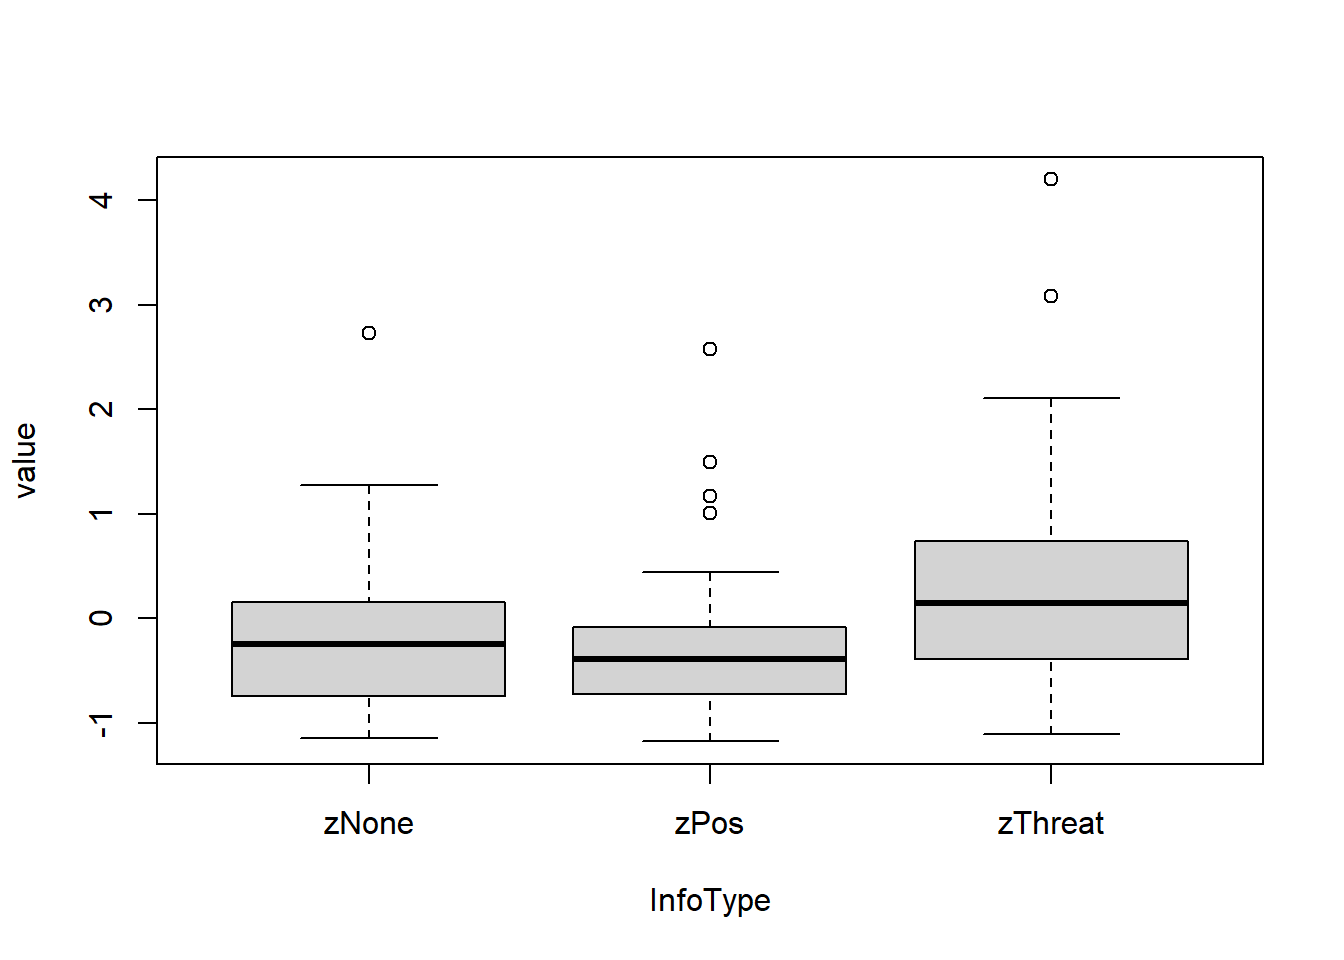
\includegraphics[width=0.5\linewidth,height=0.5\textheight]{03-Robust-Samples_files/figure-latex/Dependent-t-test-Plots-1} \end{center}

\begin{Shaded}
\begin{Highlighting}[]
\NormalTok{    DF }\OtherTok{\textless{}{-}}\NormalTok{ fieldWide }\SpecialCharTok{\%\textgreater{}\%} \FunctionTok{gather}\NormalTok{(InfoType, value, }\DecValTok{2}\SpecialCharTok{:}\DecValTok{4}\NormalTok{) }\CommentTok{\# or change to Long}
\NormalTok{    DF}\SpecialCharTok{$}\NormalTok{InfoType }\OtherTok{\textless{}{-}} \FunctionTok{as.factor}\NormalTok{(DF}\SpecialCharTok{$}\NormalTok{InfoType)}
    \FunctionTok{boxplot}\NormalTok{(value }\SpecialCharTok{\textasciitilde{}}\NormalTok{ InfoType, DF)}
\NormalTok{  DF\_Means }\OtherTok{\textless{}{-}}\NormalTok{ DF }\SpecialCharTok{\%\textgreater{}\%} \FunctionTok{group\_by}\NormalTok{(InfoType) }\SpecialCharTok{\%\textgreater{}\%} 
              \FunctionTok{summarise\_at}\NormalTok{(}\AttributeTok{.vars =} \FunctionTok{names}\NormalTok{(.)[}\DecValTok{3}\NormalTok{],}\AttributeTok{.funs =} \FunctionTok{c}\NormalTok{(}\AttributeTok{mean=}\StringTok{"mean"}\NormalTok{))}
  \FunctionTok{barplot}\NormalTok{(mean }\SpecialCharTok{\textasciitilde{}}\NormalTok{ InfoType, DF\_Means)}
\end{Highlighting}
\end{Shaded}

\begin{center}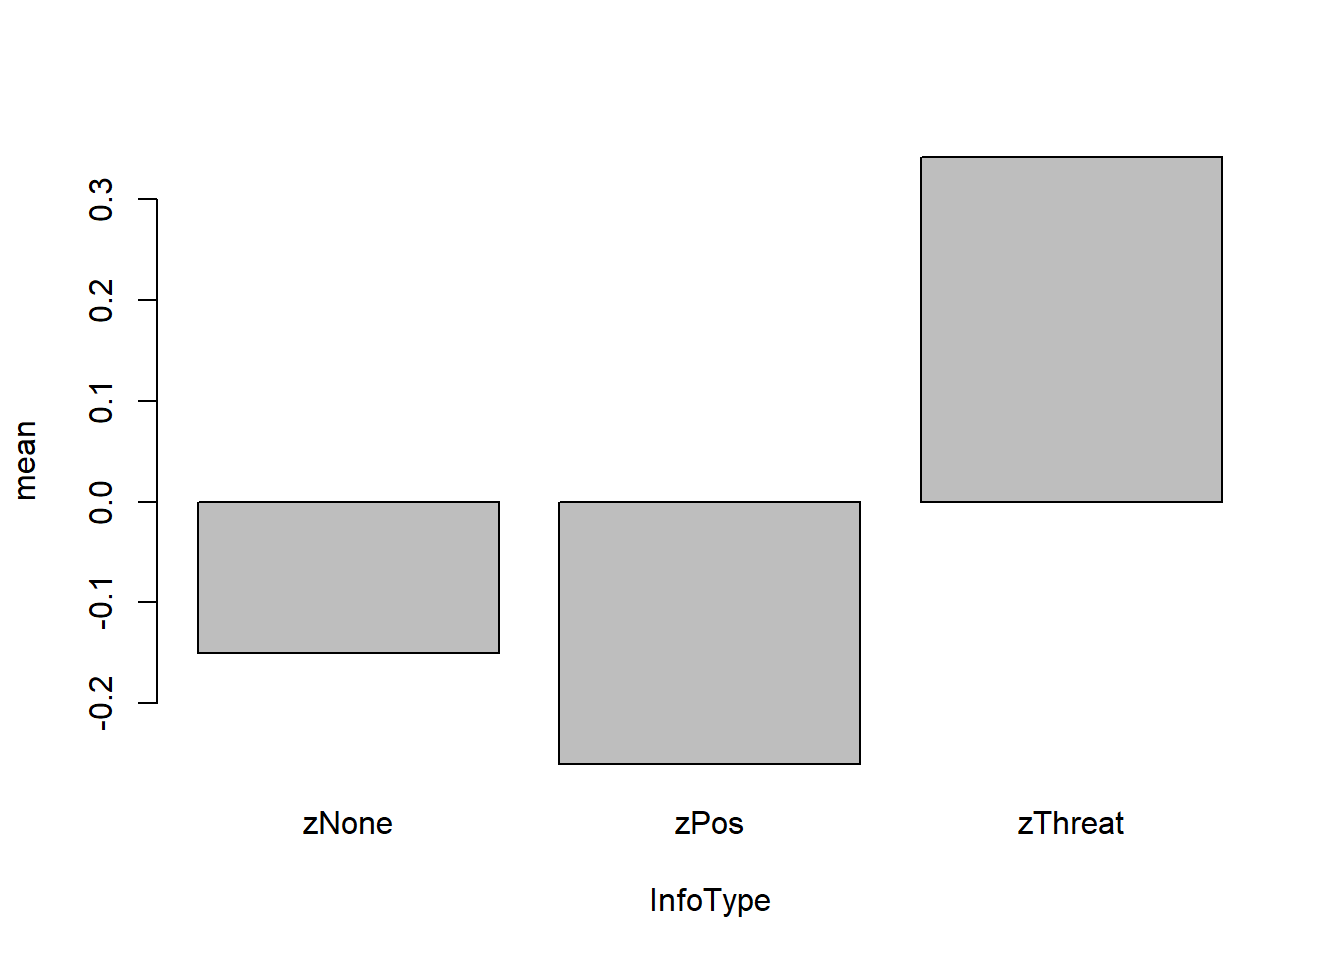
\includegraphics[width=0.5\linewidth,height=0.5\textheight]{03-Robust-Samples_files/figure-latex/Dependent-t-test-Plots-2} \end{center}

\begin{Shaded}
\begin{Highlighting}[]
  \CommentTok{\# hist(fieldWide$zThreat)}
  \CommentTok{\# hist(fieldWide$zPos)}
  \CommentTok{\# hist(fieldWide$zNone)}
\end{Highlighting}
\end{Shaded}

A valuable plot to see the distributional properties of the data is the histogram or the density plot, e.g.:

\begin{Shaded}
\begin{Highlighting}[]
    \FunctionTok{ggplot}\NormalTok{(fieldLong, }\FunctionTok{aes}\NormalTok{(}\AttributeTok{x =}\NormalTok{ value, }\AttributeTok{y =}\NormalTok{ InfoType)) }\SpecialCharTok{+}
    \FunctionTok{geom\_density\_ridges}\NormalTok{(}\FunctionTok{aes}\NormalTok{(}\AttributeTok{fill =}\NormalTok{ InfoType)) }\SpecialCharTok{+}
    \FunctionTok{scale\_fill\_manual}\NormalTok{(}\AttributeTok{values =} \FunctionTok{c}\NormalTok{(}\StringTok{"\#00AFBB"}\NormalTok{, }\StringTok{"\#E7B800"}\NormalTok{, }\StringTok{"\#FC4E07"}\NormalTok{)) }\SpecialCharTok{+} 
      \FunctionTok{theme\_bw}\NormalTok{()}
\end{Highlighting}
\end{Shaded}

\begin{center}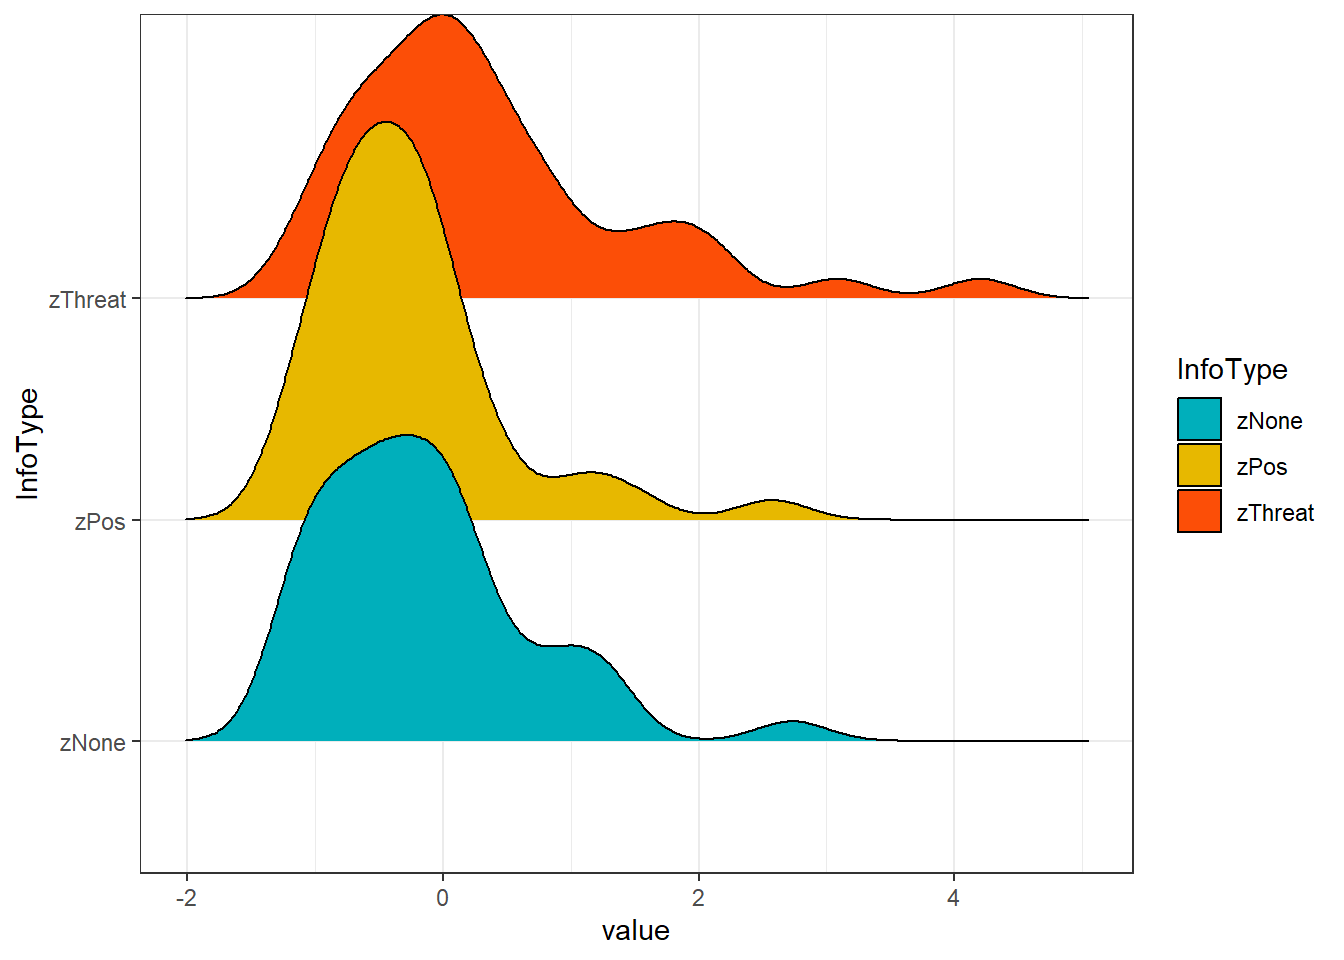
\includegraphics[width=0.5\linewidth,height=0.5\textheight]{03-Robust-Samples_files/figure-latex/Dependent-Distribution-1} \end{center}

\subsection*{Standard t-Test}\label{standard-t-test-1}
\addcontentsline{toc}{subsection}{Standard t-Test}

Calculate the standard parametric t-Test for repeatet measure designs and discuss the results.

\begin{Shaded}
\begin{Highlighting}[]
  \FunctionTok{pander}\NormalTok{(}\FunctionTok{t.test}\NormalTok{(fieldWide}\SpecialCharTok{$}\NormalTok{zThreat, fieldWide}\SpecialCharTok{$}\NormalTok{zNone, }\AttributeTok{paired =}\NormalTok{ T), }\AttributeTok{digits =} \DecValTok{3}\NormalTok{)}
\end{Highlighting}
\end{Shaded}

\begin{longtable}[]{@{}
  >{\centering\arraybackslash}p{(\columnwidth - 8\tabcolsep) * \real{0.2125}}
  >{\centering\arraybackslash}p{(\columnwidth - 8\tabcolsep) * \real{0.0625}}
  >{\centering\arraybackslash}p{(\columnwidth - 8\tabcolsep) * \real{0.1875}}
  >{\centering\arraybackslash}p{(\columnwidth - 8\tabcolsep) * \real{0.3125}}
  >{\centering\arraybackslash}p{(\columnwidth - 8\tabcolsep) * \real{0.2250}}@{}}
\caption{Paired t-test: \texttt{fieldWide\$zThreat} and \texttt{fieldWide\$zNone}}\tabularnewline
\toprule\noalign{}
\begin{minipage}[b]{\linewidth}\centering
Test statistic
\end{minipage} & \begin{minipage}[b]{\linewidth}\centering
df
\end{minipage} & \begin{minipage}[b]{\linewidth}\centering
P value
\end{minipage} & \begin{minipage}[b]{\linewidth}\centering
Alternative hypothesis
\end{minipage} & \begin{minipage}[b]{\linewidth}\centering
mean difference
\end{minipage} \\
\midrule\noalign{}
\endfirsthead
\toprule\noalign{}
\begin{minipage}[b]{\linewidth}\centering
Test statistic
\end{minipage} & \begin{minipage}[b]{\linewidth}\centering
df
\end{minipage} & \begin{minipage}[b]{\linewidth}\centering
P value
\end{minipage} & \begin{minipage}[b]{\linewidth}\centering
Alternative hypothesis
\end{minipage} & \begin{minipage}[b]{\linewidth}\centering
mean difference
\end{minipage} \\
\midrule\noalign{}
\endhead
\bottomrule\noalign{}
\endlastfoot
2.87 & 42 & 0.006405 * * & two.sided & 0.492 \\
\end{longtable}

\subsection*{Robust t-Test}\label{robust-t-test-1}
\addcontentsline{toc}{subsection}{Robust t-Test}

Next we will look at the Yuen's modified t-Test for trimmed means (\citeproc{ref-Yuen.1974}{Yuen 1974}). For an extented version with bootstrapping refer to (\citeproc{ref-Keselman.2004}{Keselman 2004})

\begin{Shaded}
\begin{Highlighting}[]
  \FunctionTok{pander}\NormalTok{(}\FunctionTok{yuend}\NormalTok{(fieldWide}\SpecialCharTok{$}\NormalTok{zThreat, fieldWide}\SpecialCharTok{$}\NormalTok{zNone, }\AttributeTok{tr =} \FloatTok{0.2}\NormalTok{), }\AttributeTok{digits =} \DecValTok{3}\NormalTok{)}
\end{Highlighting}
\end{Shaded}

\begin{itemize}
\tightlist
\item
  \textbf{test}: \emph{2.528}
\item
  \textbf{conf.int}: \emph{0.0756} and \emph{0.7335}
\item
  \textbf{se}: \emph{0.16}
\item
  \textbf{p.value}: \emph{0.01789}
\item
  \textbf{df}: \emph{26}
\item
  \textbf{diff}: \emph{0.4046}
\item
  \textbf{effsize}: \emph{0.3321}
\item
  \textbf{call}: \texttt{yuend(x\ =\ fieldWide\$zThreat,\ y\ =\ fieldWide\$zNone,\ tr\ =\ 0.2)}
\end{itemize}

\begin{Shaded}
\begin{Highlighting}[]
  \FunctionTok{set.seed}\NormalTok{(}\DecValTok{123}\NormalTok{)}
  \FunctionTok{pander}\NormalTok{(}\FunctionTok{Dqcomhd}\NormalTok{(fieldWide}\SpecialCharTok{$}\NormalTok{zThreat, fieldWide}\SpecialCharTok{$}\NormalTok{zNone, }\AttributeTok{nboot =} \DecValTok{200}\NormalTok{, }\AttributeTok{q =} \FunctionTok{c}\NormalTok{(}\FloatTok{0.25}\NormalTok{, }\FloatTok{0.5}\NormalTok{, }\FloatTok{0.75}\NormalTok{)),  }\AttributeTok{digits =} \DecValTok{3}\NormalTok{)}
\end{Highlighting}
\end{Shaded}

\begin{itemize}
\item
  \textbf{partable}:

  \begin{longtable}[]{@{}
    >{\centering\arraybackslash}p{(\columnwidth - 18\tabcolsep) * \real{0.0787}}
    >{\centering\arraybackslash}p{(\columnwidth - 18\tabcolsep) * \real{0.0562}}
    >{\centering\arraybackslash}p{(\columnwidth - 18\tabcolsep) * \real{0.0562}}
    >{\centering\arraybackslash}p{(\columnwidth - 18\tabcolsep) * \real{0.1124}}
    >{\centering\arraybackslash}p{(\columnwidth - 18\tabcolsep) * \real{0.1124}}
    >{\centering\arraybackslash}p{(\columnwidth - 18\tabcolsep) * \real{0.1461}}
    >{\centering\arraybackslash}p{(\columnwidth - 18\tabcolsep) * \real{0.1124}}
    >{\centering\arraybackslash}p{(\columnwidth - 18\tabcolsep) * \real{0.1011}}
    >{\centering\arraybackslash}p{(\columnwidth - 18\tabcolsep) * \real{0.1124}}
    >{\centering\arraybackslash}p{(\columnwidth - 18\tabcolsep) * \real{0.1124}}@{}}
  \toprule\noalign{}
  \begin{minipage}[b]{\linewidth}\centering
  q
  \end{minipage} & \begin{minipage}[b]{\linewidth}\centering
  n1
  \end{minipage} & \begin{minipage}[b]{\linewidth}\centering
  n2
  \end{minipage} & \begin{minipage}[b]{\linewidth}\centering
  est1
  \end{minipage} & \begin{minipage}[b]{\linewidth}\centering
  est2
  \end{minipage} & \begin{minipage}[b]{\linewidth}\centering
  est1-est.2
  \end{minipage} & \begin{minipage}[b]{\linewidth}\centering
  ci.low
  \end{minipage} & \begin{minipage}[b]{\linewidth}\centering
  ci.up
  \end{minipage} & \begin{minipage}[b]{\linewidth}\centering
  p.crit
  \end{minipage} & \begin{minipage}[b]{\linewidth}\centering
  p.value
  \end{minipage} \\
  \midrule\noalign{}
  \endhead
  \bottomrule\noalign{}
  \endlastfoot
  0.25 & 43 & 43 & -0.4243 & -0.7578 & 0.3335 & 0.01017 & 0.6655 & 0.05 & 0.03 \\
  0.5 & 43 & 43 & 0.1021 & -0.2668 & 0.3688 & 0.07493 & 0.685 & 0.01667 & 0 \\
  0.75 & 43 & 43 & 0.8274 & 0.2319 & 0.5956 & 0.1083 & 1.198 & 0.025 & 0.03 \\
  \end{longtable}
\item
  \textbf{call}: \texttt{Dqcomhd(x\ =\ fieldWide\$zThreat,\ y\ =\ fieldWide\$zNone,\ q\ =\ c(0.25,\ \ \ \ \ \ 0.5,\ 0.75),\ nboot\ =\ 200)}
\end{itemize}

\begin{Shaded}
\begin{Highlighting}[]
  \FunctionTok{set.seed}\NormalTok{(}\DecValTok{123}\NormalTok{)}
  \FunctionTok{pander}\NormalTok{(}\FunctionTok{dep.effect}\NormalTok{(fieldWide}\SpecialCharTok{$}\NormalTok{zThreat, fieldWide}\SpecialCharTok{$}\NormalTok{zNone))}
\end{Highlighting}
\end{Shaded}

\begin{longtable}[]{@{}
  >{\centering\arraybackslash}p{(\columnwidth - 14\tabcolsep) * \real{0.2466}}
  >{\centering\arraybackslash}p{(\columnwidth - 14\tabcolsep) * \real{0.0959}}
  >{\centering\arraybackslash}p{(\columnwidth - 14\tabcolsep) * \real{0.1233}}
  >{\centering\arraybackslash}p{(\columnwidth - 14\tabcolsep) * \real{0.0959}}
  >{\centering\arraybackslash}p{(\columnwidth - 14\tabcolsep) * \real{0.0959}}
  >{\centering\arraybackslash}p{(\columnwidth - 14\tabcolsep) * \real{0.0959}}
  >{\centering\arraybackslash}p{(\columnwidth - 14\tabcolsep) * \real{0.1233}}
  >{\centering\arraybackslash}p{(\columnwidth - 14\tabcolsep) * \real{0.1233}}@{}}
\toprule\noalign{}
\begin{minipage}[b]{\linewidth}\centering
~
\end{minipage} & \begin{minipage}[b]{\linewidth}\centering
NULL
\end{minipage} & \begin{minipage}[b]{\linewidth}\centering
Est
\end{minipage} & \begin{minipage}[b]{\linewidth}\centering
S
\end{minipage} & \begin{minipage}[b]{\linewidth}\centering
M
\end{minipage} & \begin{minipage}[b]{\linewidth}\centering
L
\end{minipage} & \begin{minipage}[b]{\linewidth}\centering
ci.low
\end{minipage} & \begin{minipage}[b]{\linewidth}\centering
ci.up
\end{minipage} \\
\midrule\noalign{}
\endhead
\bottomrule\noalign{}
\endlastfoot
\textbf{AKP} & 0 & 0.3869 & 0.1 & 0.3 & 0.5 & 0.1349 & 0.7173 \\
\textbf{QS (median)} & 0.5 & 0.7209 & 0.54 & 0.62 & 0.69 & 0.5116 & 0.814 \\
\textbf{QStr} & 0.5 & 0.6977 & 0.54 & 0.62 & 0.69 & 0.5349 & 0.7907 \\
\textbf{SIGN} & 0.5 & 0.3256 & 0.46 & 0.38 & 0.31 & 0.192 & 0.476 \\
\end{longtable}

\begin{Shaded}
\begin{Highlighting}[]
  \DocumentationTok{\#\#\#\#\#\#\#\#\#\#\#\#\#\#\#\#\#\#\#\#\#\#\#\#\#\#\#\#\#\#\#\#\#\#\#\#\#\#\#\#\#\#\#\#\#\#\#}
\end{Highlighting}
\end{Shaded}

Both tests yield significant differences. Note that trimming reduces:

\begin{enumerate}
\def\labelenumi{\arabic{enumi}.}
\tightlist
\item
  the mean difference from 0.49 to 0.40, and
\item
  the test statistic is smaller in the robust version.
\end{enumerate}

We could report the robust test as a significant difference between trimmed mean approach times to the threat and control animals, \(M_{diff} = 0.40 \ [0.08, 0.74], \ Y_t (26) = 2.53, p = 0.018\).

\section*{One-way RM-ANOVA}\label{one-way-rm-anova}
\addcontentsline{toc}{section}{One-way RM-ANOVA}

The data used in this example is the same as for the dependent t-Test (i.e.: \emph{FieldLawson2003.csv})

\subsection*{Check Assumptions}\label{check-assumptions-1}
\addcontentsline{toc}{subsection}{Check Assumptions}

To compare the latencies for all three boxes, we could use a repeated measure ANOVA function such as the \texttt{aov()}, or as an alternative the \texttt{rstatix::anova\_test()} function. But before we do the analysis, we should check for possible violations of the assumptions:

\begin{Shaded}
\begin{Highlighting}[]
  \CommentTok{\# Assumption check}
\NormalTok{  fieldLong          }\OtherTok{\textless{}{-}}\NormalTok{ fieldLong[,}\DecValTok{2}\SpecialCharTok{:}\DecValTok{4}\NormalTok{]}
\NormalTok{  fieldLong}\SpecialCharTok{$}\NormalTok{id       }\OtherTok{\textless{}{-}} \FunctionTok{factor}\NormalTok{(fieldLong}\SpecialCharTok{$}\NormalTok{id)}
\NormalTok{  fieldLong}\SpecialCharTok{$}\NormalTok{InfoType }\OtherTok{\textless{}{-}} \FunctionTok{factor}\NormalTok{(fieldLong}\SpecialCharTok{$}\NormalTok{InfoType)}
  \FunctionTok{pander}\NormalTok{(fieldLong }\SpecialCharTok{\%\textgreater{}\%} \FunctionTok{group\_by}\NormalTok{(InfoType) }\SpecialCharTok{\%\textgreater{}\%} \FunctionTok{identify\_outliers}\NormalTok{(value))}
\end{Highlighting}
\end{Shaded}

\begin{longtable}[]{@{}
  >{\centering\arraybackslash}p{(\columnwidth - 8\tabcolsep) * \real{0.1528}}
  >{\centering\arraybackslash}p{(\columnwidth - 8\tabcolsep) * \real{0.1111}}
  >{\centering\arraybackslash}p{(\columnwidth - 8\tabcolsep) * \real{0.1111}}
  >{\centering\arraybackslash}p{(\columnwidth - 8\tabcolsep) * \real{0.1806}}
  >{\centering\arraybackslash}p{(\columnwidth - 8\tabcolsep) * \real{0.1806}}@{}}
\toprule\noalign{}
\begin{minipage}[b]{\linewidth}\centering
InfoType
\end{minipage} & \begin{minipage}[b]{\linewidth}\centering
id
\end{minipage} & \begin{minipage}[b]{\linewidth}\centering
value
\end{minipage} & \begin{minipage}[b]{\linewidth}\centering
is.outlier
\end{minipage} & \begin{minipage}[b]{\linewidth}\centering
is.extreme
\end{minipage} \\
\midrule\noalign{}
\endhead
\bottomrule\noalign{}
\endlastfoot
zNone & bku59 & 2.729 & TRUE & FALSE \\
zPos & wdd2 & 2.574 & TRUE & TRUE \\
zPos & inl37 & 1.491 & TRUE & FALSE \\
zPos & vxp18 & 1.008 & TRUE & FALSE \\
zPos & pap44 & 1.166 & TRUE & FALSE \\
zThreat & tat36 & 4.2 & TRUE & TRUE \\
zThreat & gtu30 & 3.085 & TRUE & FALSE \\
\end{longtable}

\begin{Shaded}
\begin{Highlighting}[]
  \FunctionTok{pander}\NormalTok{(}\FunctionTok{rbind}\NormalTok{(}\FunctionTok{shapiro\_test}\NormalTok{(fieldWide}\SpecialCharTok{$}\NormalTok{zThreat), }
               \FunctionTok{shapiro\_test}\NormalTok{(fieldWide}\SpecialCharTok{$}\NormalTok{zPos), }
               \FunctionTok{shapiro\_test}\NormalTok{(fieldWide}\SpecialCharTok{$}\NormalTok{zNone)))}
\end{Highlighting}
\end{Shaded}

\begin{longtable}[]{@{}
  >{\centering\arraybackslash}p{(\columnwidth - 4\tabcolsep) * \real{0.2778}}
  >{\centering\arraybackslash}p{(\columnwidth - 4\tabcolsep) * \real{0.1667}}
  >{\centering\arraybackslash}p{(\columnwidth - 4\tabcolsep) * \real{0.1667}}@{}}
\toprule\noalign{}
\begin{minipage}[b]{\linewidth}\centering
variable
\end{minipage} & \begin{minipage}[b]{\linewidth}\centering
statistic
\end{minipage} & \begin{minipage}[b]{\linewidth}\centering
p.value
\end{minipage} \\
\midrule\noalign{}
\endhead
\bottomrule\noalign{}
\endlastfoot
fieldWide\$zThreat & 0.8894 & 0.0006053 \\
fieldWide\$zPos & 0.8463 & 4.207e-05 \\
fieldWide\$zNone & 0.9047 & 0.001741 \\
\end{longtable}

\begin{Shaded}
\begin{Highlighting}[]
\NormalTok{  bxp         }\OtherTok{\textless{}{-}} \FunctionTok{ggboxplot}\NormalTok{(fieldLong,}
                           \AttributeTok{x =} \StringTok{"InfoType"}\NormalTok{, }
                           \AttributeTok{y =} \StringTok{"value"}\NormalTok{, }
                           \AttributeTok{add =} \StringTok{"point"}\NormalTok{)}
  \FunctionTok{print}\NormalTok{(bxp)}
\end{Highlighting}
\end{Shaded}

\begin{center}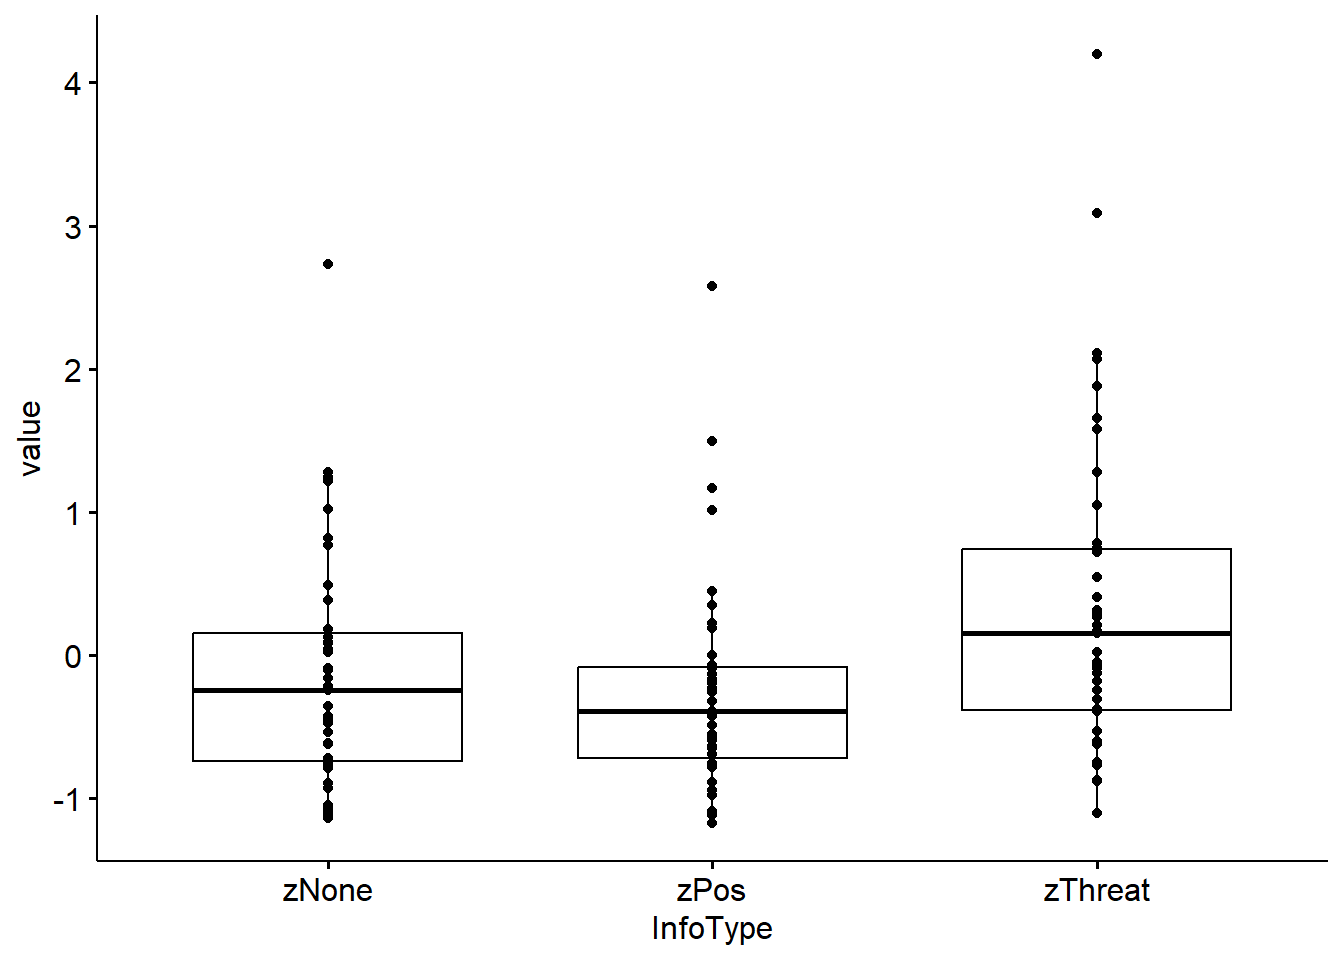
\includegraphics[width=0.5\linewidth,height=0.5\textheight]{03-Robust-Samples_files/figure-latex/ANOVA-RM-Assumption-1} \end{center}

\begin{Shaded}
\begin{Highlighting}[]
\NormalTok{  qqp         }\OtherTok{\textless{}{-}} \FunctionTok{ggqqplot}\NormalTok{(fieldLong,}
                          \StringTok{"value"}\NormalTok{,}
                          \AttributeTok{facet.by =} \StringTok{"InfoType"}\NormalTok{)}
  \FunctionTok{print}\NormalTok{(qqp)}
\end{Highlighting}
\end{Shaded}

\begin{center}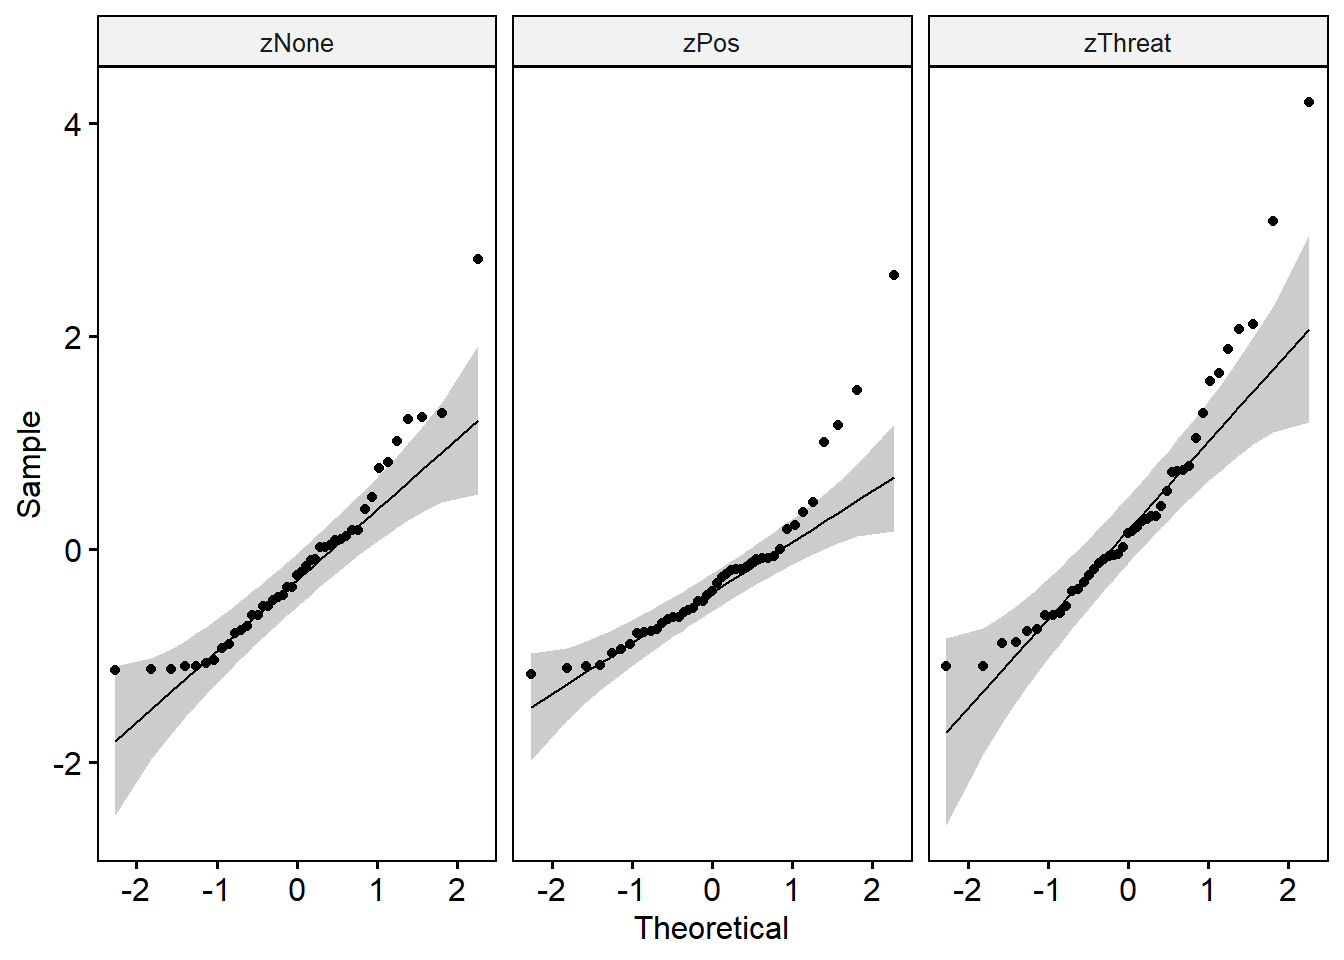
\includegraphics[width=0.5\linewidth,height=0.5\textheight]{03-Robust-Samples_files/figure-latex/ANOVA-RM-Assumption-2} \end{center}

\subsection*{Standard RM-ANOVA}\label{standard-rm-anova}
\addcontentsline{toc}{subsection}{Standard RM-ANOVA}

Since ANOVA's are special forms of linear models, we could also use the \texttt{lm()} function. The difference between these functions is the output. The \texttt{aov()} returns the table of \(F\)-statistics, whereas \texttt{lm()} returns the specific parameter estimates, significance tests and overall fit statistics.

The formula (model) of the \texttt{aov()} is specified as:

\textbf{Value \textasciitilde{} InfoType + Error(id/InfoType)}

In words: we predict the \emph{Value} from the variable \emph{InfoType} plus an \emph{error term} for that variable that is nested within the variable \emph{id}. It is the error term that tells the function that it is a repeated measures design (because the error term for the predictor variable is nested within cases).

\begin{Shaded}
\begin{Highlighting}[]
  \CommentTok{\#Non{-}robust}
  \FunctionTok{pander}\NormalTok{(}\FunctionTok{summary}\NormalTok{(}\FunctionTok{aov}\NormalTok{(value }\SpecialCharTok{\textasciitilde{}}\NormalTok{ InfoType }\SpecialCharTok{+} \FunctionTok{Error}\NormalTok{(id}\SpecialCharTok{/}\NormalTok{InfoType), }\AttributeTok{data =}\NormalTok{ fieldLong)))}
\end{Highlighting}
\end{Shaded}

\begin{longtable}[]{@{}
  >{\centering\arraybackslash}p{(\columnwidth - 10\tabcolsep) * \real{0.2361}}
  >{\centering\arraybackslash}p{(\columnwidth - 10\tabcolsep) * \real{0.0694}}
  >{\centering\arraybackslash}p{(\columnwidth - 10\tabcolsep) * \real{0.1250}}
  >{\centering\arraybackslash}p{(\columnwidth - 10\tabcolsep) * \real{0.1389}}
  >{\centering\arraybackslash}p{(\columnwidth - 10\tabcolsep) * \real{0.1389}}
  >{\centering\arraybackslash}p{(\columnwidth - 10\tabcolsep) * \real{0.1528}}@{}}
\toprule\noalign{}
\begin{minipage}[b]{\linewidth}\centering
~
\end{minipage} & \begin{minipage}[b]{\linewidth}\centering
Df
\end{minipage} & \begin{minipage}[b]{\linewidth}\centering
Sum Sq
\end{minipage} & \begin{minipage}[b]{\linewidth}\centering
Mean Sq
\end{minipage} & \begin{minipage}[b]{\linewidth}\centering
F value
\end{minipage} & \begin{minipage}[b]{\linewidth}\centering
Pr(\textgreater F)
\end{minipage} \\
\midrule\noalign{}
\endhead
\bottomrule\noalign{}
\endlastfoot
\textbf{Residuals} & 42 & 51.33 & 1.222 & NA & NA \\
\textbf{InfoType} & 2 & 8.839 & 4.42 & 7.103 & 0.001412 \\
\textbf{Residuals1} & 84 & 52.26 & 0.6222 & NA & NA \\
\end{longtable}

\begin{Shaded}
\begin{Highlighting}[]
  \CommentTok{\# Alternativ to aov(): rstatix::anova\_test()}
\NormalTok{  res.anova  }\OtherTok{\textless{}{-}} \FunctionTok{pander}\NormalTok{(}\FunctionTok{anova\_test}\NormalTok{(}\AttributeTok{data =}\NormalTok{ fieldLong,}
                                  \AttributeTok{dv =}\NormalTok{ value,}
                                  \AttributeTok{wid =}\NormalTok{ id,}
                                  \AttributeTok{within =}\NormalTok{ InfoType))}
\end{Highlighting}
\end{Shaded}

The results show means which are significantly different with latencies after threat information being significantly longer than for positive or no information. The results of the follow-up-test are shown below:

\begin{Shaded}
\begin{Highlighting}[]
  \FunctionTok{pander}\NormalTok{(}\FunctionTok{pairwise.t.test}\NormalTok{(fieldLong}\SpecialCharTok{$}\NormalTok{value, fieldLong}\SpecialCharTok{$}\NormalTok{InfoType, }\AttributeTok{p.adjust.method =} \StringTok{"bonferroni"}\NormalTok{, }\AttributeTok{paired =}\NormalTok{ T))}
\end{Highlighting}
\end{Shaded}

\begin{itemize}
\item
  \textbf{method}: paired t tests
\item
  \textbf{data.name}: fieldLong\(value and fieldLong\)InfoType
\item
  \textbf{p.value}:

  \begin{longtable}[]{@{}
    >{\centering\arraybackslash}p{(\columnwidth - 4\tabcolsep) * \real{0.1944}}
    >{\centering\arraybackslash}p{(\columnwidth - 4\tabcolsep) * \real{0.1389}}
    >{\centering\arraybackslash}p{(\columnwidth - 4\tabcolsep) * \real{0.1528}}@{}}
  \toprule\noalign{}
  \begin{minipage}[b]{\linewidth}\centering
  ~
  \end{minipage} & \begin{minipage}[b]{\linewidth}\centering
  zNone
  \end{minipage} & \begin{minipage}[b]{\linewidth}\centering
  zPos
  \end{minipage} \\
  \midrule\noalign{}
  \endhead
  \bottomrule\noalign{}
  \endlastfoot
  \textbf{zPos} & 1 & NA \\
  \textbf{zThreat} & 0.01922 & 0.005809 \\
  \end{longtable}
\item
  \textbf{p.adjust.method}: bonferroni
\end{itemize}

\subsection*{Robust ANOVA}\label{robust-anova}
\addcontentsline{toc}{subsection}{Robust ANOVA}

For the robust test we will use the \texttt{rmanovab()} function and get the post hoc tests with \texttt{pairdepb()}. The option \texttt{tr} controls the amount of trim (and the default of 20\% is advised). For the bootstrap-option the default is set to \texttt{nboot\ =\ 599} (sufficient for now, but it is common to use \texttt{nboot\ =\ 1000} or \texttt{nboot\ =\ 2000}).

\begin{Shaded}
\begin{Highlighting}[]
  \CommentTok{\#Robust}
  \FunctionTok{pander}\NormalTok{(}\FunctionTok{rmanovab}\NormalTok{(fieldLong}\SpecialCharTok{$}\NormalTok{value, fieldLong}\SpecialCharTok{$}\NormalTok{InfoType, fieldLong}\SpecialCharTok{$}\NormalTok{id, }\AttributeTok{tr =} \FloatTok{0.2}\NormalTok{, }\AttributeTok{nboot =} \DecValTok{599}\NormalTok{))}
\end{Highlighting}
\end{Shaded}

\begin{itemize}
\tightlist
\item
  \textbf{test}: \emph{6.751}
\item
  \textbf{crit}: \emph{3.439}
\item
  \textbf{call}: \texttt{rmanovab(y\ =\ fieldLong\$value,\ groups\ =\ fieldLong\$InfoType,\ blocks\ =\ fieldLong\$id,\ \ \ \ \ \ tr\ =\ 0.2,\ nboot\ =\ 599)}
\end{itemize}

The robust test results also show a significant difference between trimmed mean approach times to the three animals, \(F_t = 6.75, \ p < .050\). The results of the robust follow-up test show the difference between trimmed means (\(\hat{\psi}\)), the associated bootstrap confidence interval, the test of this difference, the critical value of the test and whether the trimmed means are significantly different (at \(\alpha = 0.05\)):

\begin{Shaded}
\begin{Highlighting}[]
  \FunctionTok{pander}\NormalTok{(}\FunctionTok{pairdepb}\NormalTok{(fieldLong}\SpecialCharTok{$}\NormalTok{value, fieldLong}\SpecialCharTok{$}\NormalTok{InfoType, fieldLong}\SpecialCharTok{$}\NormalTok{id, }\AttributeTok{tr =} \FloatTok{0.2}\NormalTok{, }\AttributeTok{nboot =} \DecValTok{599}\NormalTok{))}
\end{Highlighting}
\end{Shaded}

\begin{itemize}
\item
  \textbf{comp}:

  \begin{longtable}[]{@{}
    >{\centering\arraybackslash}p{(\columnwidth - 12\tabcolsep) * \real{0.1111}}
    >{\centering\arraybackslash}p{(\columnwidth - 12\tabcolsep) * \real{0.1111}}
    >{\centering\arraybackslash}p{(\columnwidth - 12\tabcolsep) * \real{0.1389}}
    >{\centering\arraybackslash}p{(\columnwidth - 12\tabcolsep) * \real{0.1528}}
    >{\centering\arraybackslash}p{(\columnwidth - 12\tabcolsep) * \real{0.1528}}
    >{\centering\arraybackslash}p{(\columnwidth - 12\tabcolsep) * \real{0.1389}}
    >{\centering\arraybackslash}p{(\columnwidth - 12\tabcolsep) * \real{0.1389}}@{}}
  \toprule\noalign{}
  \begin{minipage}[b]{\linewidth}\centering
  Group
  \end{minipage} & \begin{minipage}[b]{\linewidth}\centering
  Group
  \end{minipage} & \begin{minipage}[b]{\linewidth}\centering
  psihat
  \end{minipage} & \begin{minipage}[b]{\linewidth}\centering
  ci.lower
  \end{minipage} & \begin{minipage}[b]{\linewidth}\centering
  ci.upper
  \end{minipage} & \begin{minipage}[b]{\linewidth}\centering
  ~
  \end{minipage} & \begin{minipage}[b]{\linewidth}\centering
  crit
  \end{minipage} \\
  \midrule\noalign{}
  \endhead
  \bottomrule\noalign{}
  \endlastfoot
  1 & 2 & 0.5232 & 0.1599 & 0.8866 & 3.389 & 2.353 \\
  1 & 3 & 0.4046 & 0.02792 & 0.7812 & 2.528 & 2.353 \\
  2 & 3 & -0.1187 & -0.4294 & 0.192 & -0.8989 & 2.353 \\
  \end{longtable}
\item
  \textbf{fnames}: \emph{zThreat}, \emph{zPos} and \emph{zNone}
\item
  \textbf{call}: \texttt{pairdepb(y\ =\ fieldLong\$value,\ groups\ =\ fieldLong\$InfoType,\ blocks\ =\ fieldLong\$id,\ \ \ \ \ \ tr\ =\ 0.2,\ nboot\ =\ 599)}
\end{itemize}

\begin{Shaded}
\begin{Highlighting}[]
  \DocumentationTok{\#\#\#\#\#\#\#\#\#\#\#\#\#\#\#\#\#\#\#\#\#\#\#\#\#\#\#\#\#\#\#\#\#\#\#\#\#\#\#\#\#\#\#\#\#\#\#}
\end{Highlighting}
\end{Shaded}

We would report that the trimmed mean difference in latency between the threat box and the positive, \(\hat{\psi} = 0.52 \ [0.14,0.90]\), and no information, \(\hat{\psi} = 0.40 \ [0.01,0.80]\)\footnote{be cautios with the interpretation of an effect if the \(CI\) has an upper, or lower limit so close to Null!} boxes were significant. The trimmed mean difference between the positive and the no information box was not, \(\hat{\psi} = -0.12 \ [-0.44,0.90]\).

\section*{Regression Models}\label{regression-models}
\addcontentsline{toc}{section}{Regression Models}

Download the data for this example \emph{FieldCH2008.csv} from the Blackboard. The study examines the extent to which \emph{social anxiety} can be predicted from measures of \emph{worry}, \emph{shame}, \emph{visual imagery} and \emph{obsessive beliefs}.

The example demonstrates a standard and a robust linear model with multiple predictors (i.e., multiple regression). A subset of the data is shown in the following table:

\begin{Shaded}
\begin{Highlighting}[]
\NormalTok{  fieldCH }\OtherTok{\textless{}{-}} \FunctionTok{read\_csv}\NormalTok{(}\StringTok{"Daten/FieldCH2008.csv"}\NormalTok{)}
  \FunctionTok{head}\NormalTok{(fieldCH)}
\end{Highlighting}
\end{Shaded}

\begin{verbatim}
## # A tibble: 6 x 6
##      id socAnx worry shame imagery obsessive
##   <dbl>  <dbl> <dbl> <dbl>   <dbl>     <dbl>
## 1     1     36    64  151       68       319
## 2     2     24    41  139.      73       158
## 3     3    106    78  179      104       421
## 4     4     42    37  147.      58       221
## 5     5     55    49  158       88       332
## 6     6     77    62  165      118       255
\end{verbatim}

\subsection*{Check Data}\label{check-data}
\addcontentsline{toc}{subsection}{Check Data}

Before running a regression model we should have a closer look at the correlations between all the variables of the model. One very convinient way to do this is to use the \texttt{corrplot()} function:

\begin{Shaded}
\begin{Highlighting}[]
\NormalTok{  A }\OtherTok{\textless{}{-}} \FunctionTok{na.omit}\NormalTok{(fieldCH[,}\DecValTok{2}\SpecialCharTok{:}\DecValTok{6}\NormalTok{])}
\NormalTok{  CorrMat }\OtherTok{\textless{}{-}} \FunctionTok{cor}\NormalTok{(A)}
  \FunctionTok{corrplot.mixed}\NormalTok{(CorrMat, }\AttributeTok{upper =} \StringTok{"ellipse"}\NormalTok{, }\AttributeTok{lower =} \StringTok{"number"}\NormalTok{,}
                 \AttributeTok{tl.pos =} \StringTok{"lt"}\NormalTok{, }\AttributeTok{tl.col =} \StringTok{"black"}\NormalTok{, }\AttributeTok{tl.offset=}\DecValTok{1}\NormalTok{, }\AttributeTok{tl.srt =} \DecValTok{0}\NormalTok{)  }
\end{Highlighting}
\end{Shaded}

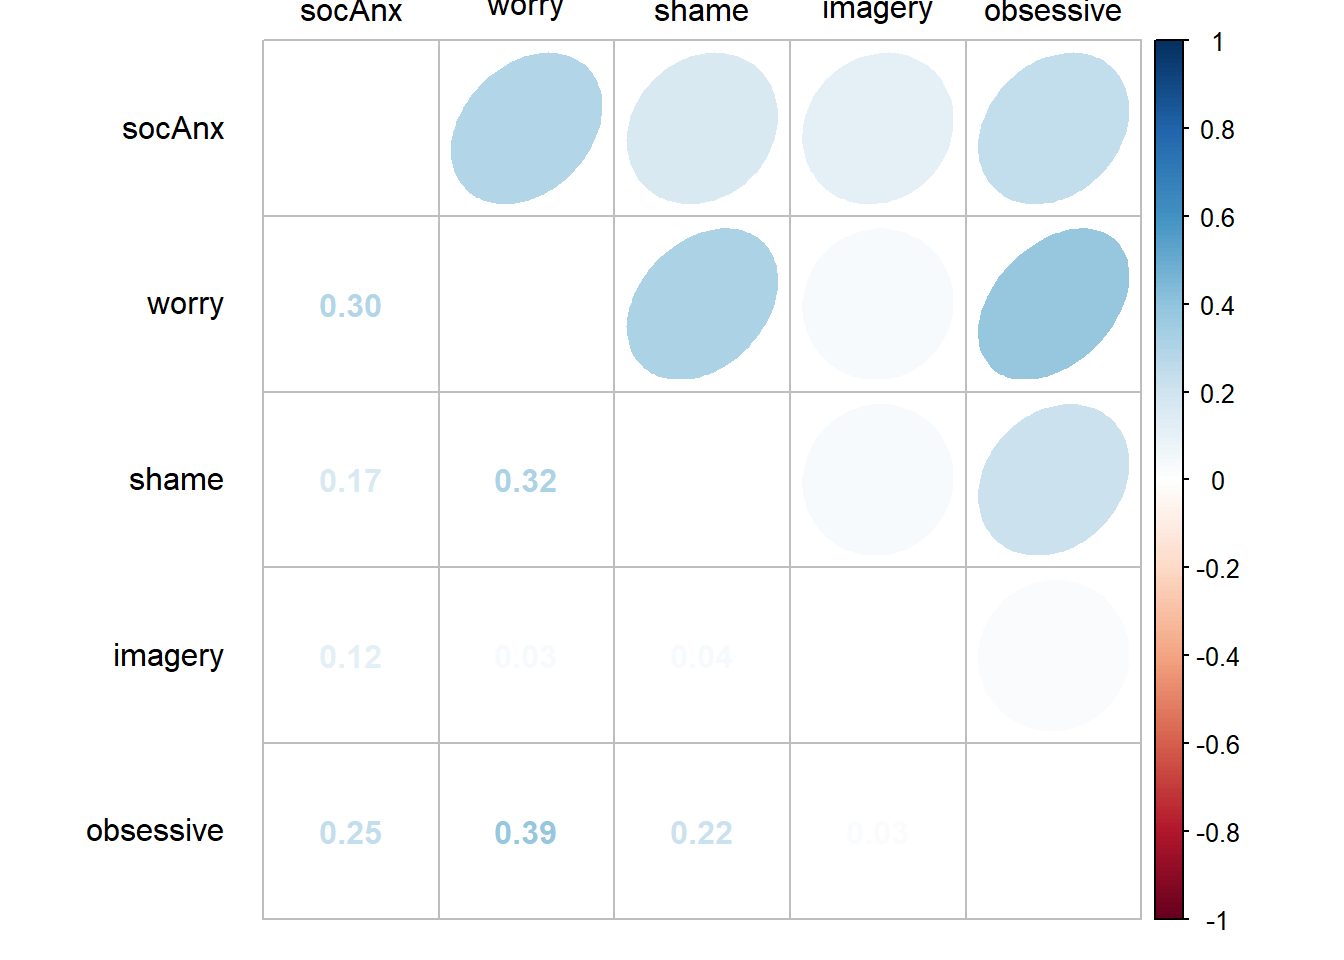
\includegraphics{03-Robust-Samples_files/figure-latex/Linear-Model-Data-Corr-1.pdf}

Scatter-Plots are also a good way to get a better insight in the beahaviour of your data:

\begin{figure}
\centering
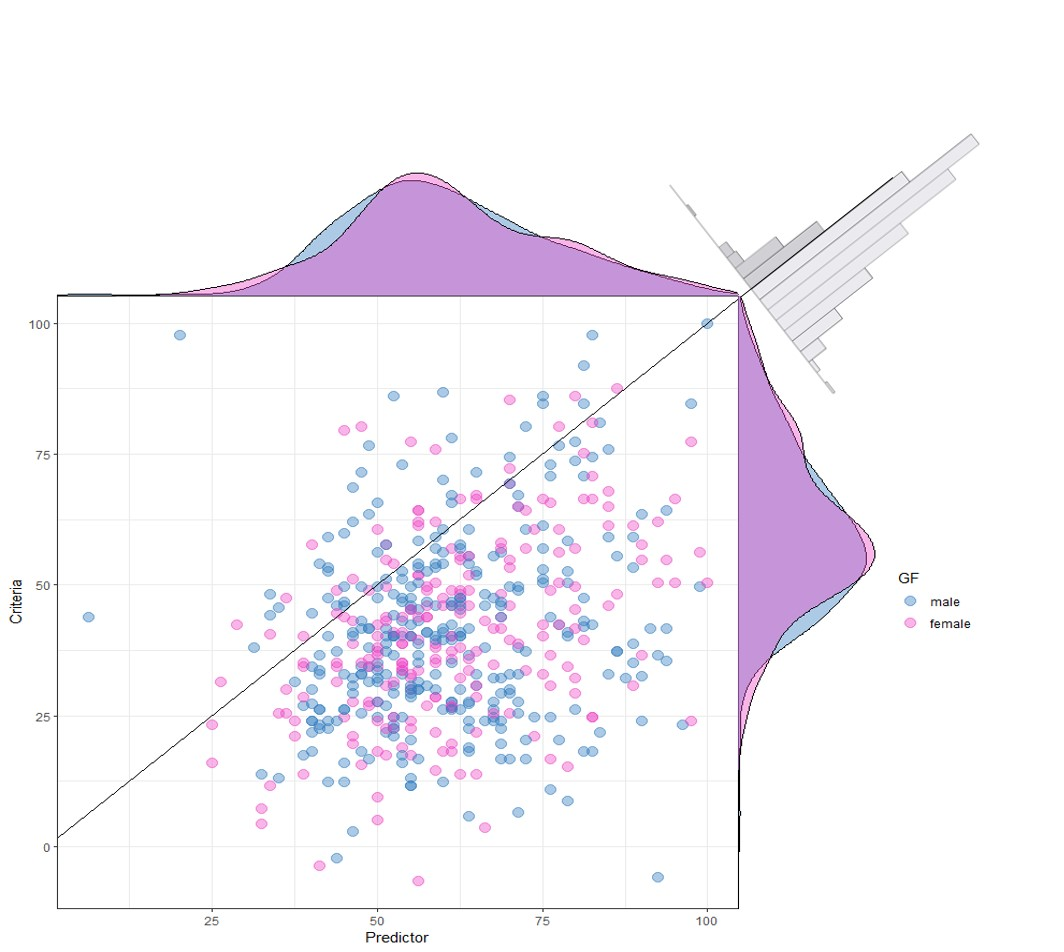
\includegraphics{Images/UltimateScatterPlot.jpg}
\caption{Figure: Scatterplot for data-check}
\end{figure}

Again, many different routines and functions are available to check for the assumptions of a linear model. For now we will leave it with that and turn to the linear model itself.

\subsection*{Standard Linear Model}\label{standard-linear-model}
\addcontentsline{toc}{subsection}{Standard Linear Model}

We use the \texttt{lm()} at its most basic form:

\begin{Shaded}
\begin{Highlighting}[]
\NormalTok{    socAnx.normal }\OtherTok{\textless{}{-}} \FunctionTok{lm}\NormalTok{(socAnx }\SpecialCharTok{\textasciitilde{}}\NormalTok{ worry }\SpecialCharTok{+}\NormalTok{ shame }\SpecialCharTok{+}\NormalTok{ imagery }\SpecialCharTok{+}\NormalTok{ obsessive, }\AttributeTok{data =}\NormalTok{ fieldCH)}
\NormalTok{    A }\OtherTok{\textless{}{-}} \FunctionTok{summary}\NormalTok{(socAnx.normal)}
    \FunctionTok{pander}\NormalTok{(}\FunctionTok{summary}\NormalTok{(socAnx.normal))}
\end{Highlighting}
\end{Shaded}

\begin{longtable}[]{@{}
  >{\centering\arraybackslash}p{(\columnwidth - 8\tabcolsep) * \real{0.2500}}
  >{\centering\arraybackslash}p{(\columnwidth - 8\tabcolsep) * \real{0.1528}}
  >{\centering\arraybackslash}p{(\columnwidth - 8\tabcolsep) * \real{0.1806}}
  >{\centering\arraybackslash}p{(\columnwidth - 8\tabcolsep) * \real{0.1389}}
  >{\centering\arraybackslash}p{(\columnwidth - 8\tabcolsep) * \real{0.1667}}@{}}
\toprule\noalign{}
\begin{minipage}[b]{\linewidth}\centering
~
\end{minipage} & \begin{minipage}[b]{\linewidth}\centering
Estimate
\end{minipage} & \begin{minipage}[b]{\linewidth}\centering
Std. Error
\end{minipage} & \begin{minipage}[b]{\linewidth}\centering
t value
\end{minipage} & \begin{minipage}[b]{\linewidth}\centering
Pr(\textgreater\textbar t\textbar)
\end{minipage} \\
\midrule\noalign{}
\endhead
\bottomrule\noalign{}
\endlastfoot
\textbf{(Intercept)} & 5.289 & 7.369 & 0.7177 & 0.4733 \\
\textbf{worry} & 0.4379 & 0.09484 & 4.617 & 4.946e-06 \\
\textbf{shame} & 0.05957 & 0.04145 & 1.437 & 0.1513 \\
\textbf{imagery} & 0.1216 & 0.04847 & 2.508 & 0.01245 \\
\textbf{obsessive} & 0.04917 & 0.01525 & 3.224 & 0.001346 \\
\end{longtable}

\begin{longtable}[]{@{}
  >{\centering\arraybackslash}p{(\columnwidth - 6\tabcolsep) * \real{0.2083}}
  >{\centering\arraybackslash}p{(\columnwidth - 6\tabcolsep) * \real{0.3056}}
  >{\centering\arraybackslash}p{(\columnwidth - 6\tabcolsep) * \real{0.1250}}
  >{\centering\arraybackslash}p{(\columnwidth - 6\tabcolsep) * \real{0.2361}}@{}}
\caption{Fitting linear model: socAnx \textasciitilde{} worry + shame + imagery + obsessive}\tabularnewline
\toprule\noalign{}
\begin{minipage}[b]{\linewidth}\centering
Observations
\end{minipage} & \begin{minipage}[b]{\linewidth}\centering
Residual Std. Error
\end{minipage} & \begin{minipage}[b]{\linewidth}\centering
\(R^2\)
\end{minipage} & \begin{minipage}[b]{\linewidth}\centering
Adjusted \(R^2\)
\end{minipage} \\
\midrule\noalign{}
\endfirsthead
\toprule\noalign{}
\begin{minipage}[b]{\linewidth}\centering
Observations
\end{minipage} & \begin{minipage}[b]{\linewidth}\centering
Residual Std. Error
\end{minipage} & \begin{minipage}[b]{\linewidth}\centering
\(R^2\)
\end{minipage} & \begin{minipage}[b]{\linewidth}\centering
Adjusted \(R^2\)
\end{minipage} \\
\midrule\noalign{}
\endhead
\bottomrule\noalign{}
\endlastfoot
512 & 23.26 & 0.1229 & 0.116 \\
\end{longtable}

\subsection*{Robust Linear Model (RLM)}\label{robust-linear-model-rlm}
\addcontentsline{toc}{subsection}{Robust Linear Model (RLM)}

There are several options for fitting robust regression in R. We will demonstrate the \texttt{lmrob()} function, which fits a robust variant of the social anxiety model based on an \(M\)-estimator (\citeproc{ref-Koller.2011}{Koller 2011}) using iteratively reweighted least squares (IRWLS) estimation.

This function, at its most basic, takes the same form as \texttt{lm()}, which means that we can simply replace \texttt{lm} with \texttt{lmrob} and proceed as before.

\begin{Shaded}
\begin{Highlighting}[]
\NormalTok{    socAnx.robust }\OtherTok{\textless{}{-}} \FunctionTok{lmrob}\NormalTok{(socAnx }\SpecialCharTok{\textasciitilde{}}\NormalTok{ worry }\SpecialCharTok{+}\NormalTok{ shame }\SpecialCharTok{+}\NormalTok{ imagery }\SpecialCharTok{+}\NormalTok{ obsessive, }\AttributeTok{data =}\NormalTok{ fieldCH)}
    \FunctionTok{summary}\NormalTok{(socAnx.robust)}
\end{Highlighting}
\end{Shaded}

\begin{verbatim}
## 
## Call:
## lmrob(formula = socAnx ~ worry + shame + imagery + obsessive, data = fieldCH)
##  \--> method = "MM"
## Residuals:
##      Min       1Q   Median       3Q      Max 
## -77.8329 -15.1522   0.0181  13.8852 101.7230 
## 
## Coefficients:
##             Estimate Std. Error t value Pr(>|t|)    
## (Intercept)   5.3514     7.8857    0.68  0.49769    
## worry         0.4844     0.1006    4.81    2e-06 ***
## shame         0.0259     0.0496    0.52  0.60162    
## imagery       0.1294     0.0475    2.72  0.00666 ** 
## obsessive     0.0552     0.0158    3.48  0.00054 ***
## ---
## Signif. codes:  0 '***' 0.001 '**' 0.01 '*' 0.05 '.' 0.1 ' ' 1
## 
## Robust residual standard error: 22 
##   (47 Beobachtungen als fehlend gelöscht)
## Multiple R-squared:  0.141,  Adjusted R-squared:  0.135 
## Convergence in 15 IRWLS iterations
## 
## Robustness weights: 
##  observation 222 is an outlier with |weight| <= 8.9e-06 ( < 0.0002); 
##  45 weights are ~= 1. The remaining 466 ones are summarized as
##    Min. 1st Qu.  Median    Mean 3rd Qu.    Max. 
##    0.17    0.87    0.95    0.90    0.98    1.00 
## Algorithmic parameters: 
##        tuning.chi                bb        tuning.psi        refine.tol 
##          1.55e+00          5.00e-01          4.69e+00          1.00e-07 
##           rel.tol         scale.tol         solve.tol          zero.tol 
##          1.00e-07          1.00e-10          1.00e-07          1.00e-10 
##       eps.outlier             eps.x warn.limit.reject warn.limit.meanrw 
##          1.95e-04          9.53e-10          5.00e-01          5.00e-01 
##      nResample         max.it       best.r.s       k.fast.s          k.max 
##            500             50              2              1            200 
##    maxit.scale      trace.lev            mts     compute.rd fast.s.large.n 
##            200              0           1000              0           2000 
##                   psi           subsampling                   cov 
##            "bisquare"         "nonsingular"         ".vcov.avar1" 
## compute.outlier.stats 
##                  "SM" 
## seed : int(0)
\end{verbatim}

Note that the \(b\)-values (now labelled \emph{Estimates}), standard errors, \(t\)-values and \(p\)-values are slightly different.

The interpretation of the model does not change substantially (worry, visual imagery and obsessive beliefs significantly predict social anxiety, shame does not) but:

\begin{quote}
the parameter estimates and associated standard error, test statistic and \(p\)-value from the robust model will have been relatively unaffected by the shape of the model residuals and outliers etc.
\end{quote}

\subsubsection*{RLM-Extended}\label{rlm-extended}
\addcontentsline{toc}{subsubsection}{RLM-Extended}

Given that our earlier examples are also variants of the linear model, we could also use the \texttt{lmrob()} function if we wanted to use an \(M\)-estimator instead of \emph{trimmed means}.

For example, the classical models that compared two independent meansand several independent means were obtained using the \texttt{aov()} function, but this function is a \emph{wrapper} for the \texttt{lm()} function that expresses the model in terms of F-statistics (as in ANOVA) rather than model parameters.

If we use the \texttt{lm()} function directly to fit these models we obtain the model parameters:

\begin{Shaded}
\begin{Highlighting}[]
    \FunctionTok{summary}\NormalTok{(}\FunctionTok{lm}\NormalTok{(z }\SpecialCharTok{\textasciitilde{}}\NormalTok{ Intervention, }\AttributeTok{data =}\NormalTok{ posInfoFBQ))}
\end{Highlighting}
\end{Shaded}

\begin{verbatim}
## 
## Call:
## lm(formula = z ~ Intervention, data = posInfoFBQ)
## 
## Residuals:
##     Min      1Q  Median      3Q     Max 
## -2.7089 -0.4072  0.0399  0.4222  2.0057 
## 
## Coefficients:
##                                  Estimate Std. Error t value Pr(>|t|)    
## (Intercept)                         0.655      0.148    4.44  3.3e-05 ***
## InterventionPositive Information   -1.442      0.206   -7.00  1.3e-09 ***
## ---
## Signif. codes:  0 '***' 0.001 '**' 0.01 '*' 0.05 '.' 0.1 ' ' 1
## 
## Residual standard error: 0.87 on 70 degrees of freedom
## Multiple R-squared:  0.412,  Adjusted R-squared:  0.403 
## F-statistic:   49 on 1 and 70 DF,  p-value: 1.26e-09
\end{verbatim}

\begin{Shaded}
\begin{Highlighting}[]
    \FunctionTok{summary}\NormalTok{(}\FunctionTok{lm}\NormalTok{(z }\SpecialCharTok{\textasciitilde{}}\NormalTok{ Intervention, }\AttributeTok{data =}\NormalTok{ fbqOnly))}
\end{Highlighting}
\end{Shaded}

\begin{verbatim}
## 
## Call:
## lm(formula = z ~ Intervention, data = fbqOnly)
## 
## Residuals:
##     Min      1Q  Median      3Q     Max 
## -2.7089 -0.4178  0.0399  0.4752  2.0057 
## 
## Coefficients:
##                                   Estimate Std. Error t value Pr(>|t|)    
## (Intercept)                          0.655      0.136    4.83  4.7e-06 ***
## InterventionNon-Anxious Modelling   -0.479      0.192   -2.50    0.014 *  
## InterventionPositive Information    -1.442      0.189   -7.62  1.2e-11 ***
## ---
## Signif. codes:  0 '***' 0.001 '**' 0.01 '*' 0.05 '.' 0.1 ' ' 1
## 
## Residual standard error: 0.8 on 104 degrees of freedom
## Multiple R-squared:  0.368,  Adjusted R-squared:  0.356 
## F-statistic: 30.3 on 2 and 104 DF,  p-value: 4.31e-11
\end{verbatim}

It is a simple matter to estimate these parameters with an M-estimator by replacing \texttt{lm} with \texttt{lmrob}:

\begin{Shaded}
\begin{Highlighting}[]
    \FunctionTok{summary}\NormalTok{(}\FunctionTok{lmrob}\NormalTok{(z }\SpecialCharTok{\textasciitilde{}}\NormalTok{ Intervention, }\AttributeTok{data =}\NormalTok{ posInfoFBQ))}
\end{Highlighting}
\end{Shaded}

\begin{verbatim}
## 
## Call:
## lmrob(formula = z ~ Intervention, data = posInfoFBQ)
##  \--> method = "MM"
## Residuals:
##     Min      1Q  Median      3Q     Max 
## -2.7796 -0.4382  0.0142  0.4031  1.9350 
## 
## Coefficients:
##                                  Estimate Std. Error t value Pr(>|t|)    
## (Intercept)                        0.6572     0.0824    7.97  2.0e-11 ***
## InterventionPositive Information  -1.3732     0.2239   -6.13  4.6e-08 ***
## ---
## Signif. codes:  0 '***' 0.001 '**' 0.01 '*' 0.05 '.' 0.1 ' ' 1
## 
## Robust residual standard error: 0.66 
## Multiple R-squared:  0.465,  Adjusted R-squared:  0.458 
## Convergence in 16 IRWLS iterations
## 
## Robustness weights: 
##  13 weights are ~= 1. The remaining 59 ones are summarized as
##    Min. 1st Qu.  Median    Mean 3rd Qu.    Max. 
##    0.04    0.75    0.94    0.84    0.97    1.00 
## Algorithmic parameters: 
##        tuning.chi                bb        tuning.psi        refine.tol 
##          1.55e+00          5.00e-01          4.69e+00          1.00e-07 
##           rel.tol         scale.tol         solve.tol          zero.tol 
##          1.00e-07          1.00e-10          1.00e-07          1.00e-10 
##       eps.outlier             eps.x warn.limit.reject warn.limit.meanrw 
##          1.39e-03          1.82e-12          5.00e-01          5.00e-01 
##      nResample         max.it       best.r.s       k.fast.s          k.max 
##            500             50              2              1            200 
##    maxit.scale      trace.lev            mts     compute.rd fast.s.large.n 
##            200              0           1000              0           2000 
##                   psi           subsampling                   cov 
##            "bisquare"         "nonsingular"         ".vcov.avar1" 
## compute.outlier.stats 
##                  "SM" 
## seed : int(0)
\end{verbatim}

\begin{Shaded}
\begin{Highlighting}[]
    \FunctionTok{summary}\NormalTok{(}\FunctionTok{lmrob}\NormalTok{(z }\SpecialCharTok{\textasciitilde{}}\NormalTok{ Intervention, }\AttributeTok{data =}\NormalTok{ fbqOnly))}
\end{Highlighting}
\end{Shaded}

\begin{verbatim}
## 
## Call:
## lmrob(formula = z ~ Intervention, data = fbqOnly)
##  \--> method = "MM"
## Residuals:
##     Min      1Q  Median      3Q     Max 
## -2.7795 -0.4527  0.0143  0.4204  1.9351 
## 
## Coefficients:
##                                   Estimate Std. Error t value Pr(>|t|)    
## (Intercept)                         0.6572     0.0823    7.98  2.0e-12 ***
## InterventionNon-Anxious Modelling  -0.4391     0.1360   -3.23   0.0017 ** 
## InterventionPositive Information   -1.3733     0.2246   -6.11  1.7e-08 ***
## ---
## Signif. codes:  0 '***' 0.001 '**' 0.01 '*' 0.05 '.' 0.1 ' ' 1
## 
## Robust residual standard error: 0.65 
## Multiple R-squared:  0.399,  Adjusted R-squared:  0.388 
## Convergence in 16 IRWLS iterations
## 
## Robustness weights: 
##  15 weights are ~= 1. The remaining 92 ones are summarized as
##    Min. 1st Qu.  Median    Mean 3rd Qu.    Max. 
##    0.03    0.86    0.94    0.87    0.98    1.00 
## Algorithmic parameters: 
##        tuning.chi                bb        tuning.psi        refine.tol 
##          1.55e+00          5.00e-01          4.69e+00          1.00e-07 
##           rel.tol         scale.tol         solve.tol          zero.tol 
##          1.00e-07          1.00e-10          1.00e-07          1.00e-10 
##       eps.outlier             eps.x warn.limit.reject warn.limit.meanrw 
##          9.35e-04          1.82e-12          5.00e-01          5.00e-01 
##      nResample         max.it       best.r.s       k.fast.s          k.max 
##            500             50              2              1            200 
##    maxit.scale      trace.lev            mts     compute.rd fast.s.large.n 
##            200              0           1000              0           2000 
##                   psi           subsampling                   cov 
##            "bisquare"         "nonsingular"         ".vcov.avar1" 
## compute.outlier.stats 
##                  "SM" 
## seed : int(0)
\end{verbatim}

\part*{PART IV: Summary}\label{part-part-iv-summary}
\addcontentsline{toc}{part}{PART IV: Summary}

\section*{Conclusions and recommendations}\label{conclusions-and-recommendations}
\addcontentsline{toc}{section}{Conclusions and recommendations}

Overall we can conclude that:

\begin{enumerate}
\def\labelenumi{\arabic{enumi}.}
\tightlist
\item
  the assumptions of the statistical models frequently used are (highly) unlikely to be met for psychological data
\item
  violating these assumptions has unpleasant and undesirable effects on the:

  \begin{itemize}
  \tightlist
  \item
    model parameters
  \item
    their associated standard errors, confidence intervals and
  \item
    p-values
  \end{itemize}
\item
  traditional methods for dealing with violations of model assumptions are (often) ineffective
\item
  there are numerous robust alternatives to the models
\item
  they are straightforward to implement
\end{enumerate}

\subsection*{Recommendations}\label{recommendations}
\addcontentsline{toc}{subsection}{Recommendations}

The possible \textbf{practical consequences} of violating assumptions include:

\begin{itemize}
\tightlist
\item
  relatively low power
\item
  inaccurate confidence intervals
\item
  inaccurate measures of effect size (that miss important differences)
\end{itemize}

Given Micceri's findings (\citeproc{ref-Micceri.1989}{Micceri 1989}) and according to the paper of Field and Wilcox (\citeproc{ref-FieldWilcox.2017}{\&. W. Field A. P. 2017}) it seems highly improbable that every paper not explicitly demonstrating that model assumptions have been met have, in reality, met the model assumptions. Hence, following recommondations are given:

\begin{itemize}
\tightlist
\item
  Scientists, reviewers and editors should assume that assumptions have not been met unless there is an explicit and compelling statement.
\item
  It must be backed up by evidence, that the assumptions of the models fit have been met, but it is not recommend that these statements are based upon significance tests of assumptions\footnote{ because, under general conditions, such tests do not have enough power to detect violations of assumptions that have practical consequences (\citeproc{ref-Kesleman.2016}{Kesleman 2016}).}
\item
  \textbf{Currently the best way} of investigating the impact of violations of model assumptions is to \textbf{use a modern robust method and compare the results to the standard model}. If the assumptions are met, the expectation is that they will give consistent results. Otherwise, the conventional method is in doubt.
\item
  Do not rely on large sample size!

  \begin{itemize}
  \tightlist
  \item
    Heavy tail problems (\citeproc{ref-Micceri.1989}{Micceri 1989})\footnote{ he studied the distributional characteristics of 440 large-sample psychology-relevant measures. Remarkably, when looking at tail weight only 15.2\% approximated a normal distribution and nearly 67\% had at least one tail that was moderately to extremely heavy. In terms of symmetry, only 28.4\% approximated a normal distribution with the remainder moderately to extremely skewed. Looking at both symmetry and tail weight together only 6.8\% of the 440 distributions approximated normality. These data show that tail weight and symmetry consistent with a normal distribution is extremely rare in psychological data.}
  \item
    Skew problems\footnote{ poor control over the Type I error probability can occur even with large sample sizes. Imagine a two-sample Student's T, \(N_1 = 400, sd = 1\), \textbf{sampling distribution = lognormal} distribution. \(N_2= 1000, sd = 1\), \textbf{sampling distribution = normal}. The Type I error probability is approximately \textbf{0.14} rather than the nominal 0.05 \(\rightarrow\) regardless of how large the sample size might be, results can be misleading.}
  \end{itemize}
\item
  insist on sensitivity analysis for all frequentist analyses, i.e.~non-robust estimators (such as OLS and ML) are compared to a robust variant. Where the two models yield ostensibly the same results then either model may be reported, where the models deviate substantially then the robust model should be reported unless a compelling evidence-based case can be made that model assumptions have been met.
\item
  when for a certain problem a specific test is unavailable, it should be technically possible to bootstrap standard errors and confidence intervals from pretty much any model.
\item
  statements along the lines of `ANOVA/regression/the t-test is robust' should be banned!
\end{itemize}

\phantomsection\label{refs}
\begin{CSLReferences}{1}{0}
\bibitem[\citeproctext]{ref-Brunner.2002}
Brunner E., Langer F., Domhof S. 2002. \emph{Nonparametric Analysis of Longitudinal Data in Factorial Experiments.} {John Wiley \& Sons, New York.}

\bibitem[\citeproctext]{ref-FieldLawson.2003}
Field, \& Lawson, A. P. 2003. {``Fear Information and the Development of Fears During Childhood: Effects on Implicit Fear Responses and Behavioural Avoidance.''} \emph{Behaviour Research and Therapy, 41(11), 1277-1293}. \url{https://doi.org/10.1016/s0005-7967(03)00034-2}.

\bibitem[\citeproctext]{ref-FieldWilcox.2017}
Field, \& Wilcox, A. P. 2017. {``Robust Statistical Methods: A Primer for Clinical Psychology and Experimental Psychopathology Researchers.''} \emph{Behaviour Research and Therapy, 98, 19-38}. https://doi.org/\url{https://doi.org/10.1016/j.brat.2017.05.013}.

\bibitem[\citeproctext]{ref-Hurn.2008}
Hurn, M. David. 2008. {``Modern Robust Statistical Methods: An Easy Way to Maximize the Accuracy and Power of Your Research.''} \emph{American Psychologist, Vol. 63, No. 7, 591--601}. \url{https://doi.org/10.1037/0003-066X.63.7.591}.

\bibitem[\citeproctext]{ref-Kelly.2010}
Kelly, Barker, V. L. 2010. {``Can Rachman's Indirect Pathways Be Used to Un-Learn Fear? A Prospective Paradigm to Test Whether Children's Fears Can Be Reduced Using Positive Information and Modelling a Non-Anxious Response.''} \emph{Behaviour Research and Therapy, 48(2), 164-170}. \url{https://doi.org/10.1016/j.brat.2009.10.002}.

\bibitem[\citeproctext]{ref-Keselman.2004}
Keselman, H. J. 2004. {``The New and Improved Two-Sample t Test.''} \emph{American Psychological Society, 15(1), 47-51}. \url{https://doi.org/10.1111/j.0963-7214.2004.01501008.x}.

\bibitem[\citeproctext]{ref-Kesleman.2016}
Kesleman, Othman, H. J. 2016. {``Generalized Linear Model Analyses for Treatment Group Equality When Data Are Non-Normal.''} \emph{Journal of Modern Applied Statistical Methods, 15(1), 32-61}. https://doi.org/\url{http://dx.doi.org/10.1037//0033-2909.105.1.156}.

\bibitem[\citeproctext]{ref-Koller.2011}
Koller, \& Stahel, M. 2011. {``Sharpening Wald-Type Inference in Robust Regression for Small Samples.''} \emph{Computational Statistics \& Data Analysis, 58(8), 2504-2515}. https://doi.org/\url{http://dx.doi.org/10.1016/j.csda.2011.02.014}.

\bibitem[\citeproctext]{ref-Mair.2020}
Mair, Wilcox R., P. 2020. {``Robust Statistical Methods in r Using the WRS2 Package.''} \emph{Behavioural Research Methods, 52(2), 464-488}. \url{https://doi.org/10.3758/s13428-019-01246-w}.

\bibitem[\citeproctext]{ref-Micceri.1989}
Micceri, T. 1989. {``The Unicorn, the Normal Curve, and Other Improbable Creatures.''} \emph{Psychological Bulletin, 105(1), 156-166}. https://doi.org/\url{http://dx.doi.org/10.1037//0033-2909.105.1.156}.

\bibitem[\citeproctext]{ref-Tukey.1960}
Tukey, John W. 2009. \emph{A Survey of Sampling from Contaminated Distributions.} {Princeton, New Jersey: Princeton University}.

\bibitem[\citeproctext]{ref-Wilcox.2012}
Wilcox, R. 2012. \emph{Introduction to Robust Estimation \& Hypothesis Testing.} 3rd ed. Amsterdam, The Netherlands: {Elsevier}.

\bibitem[\citeproctext]{ref-Yuen.1974}
Yuen, K. K. 1974. {``2-Sample Trimmed t for Unequal Population Variances.''} \emph{Biometrika, 61(1), 165-170}. https://doi.org/\url{http://dx.doi.org/10.1093/biomet/61.1.165}.

\end{CSLReferences}

\end{document}
